%% This is the ctufit-thesis example file. It is used to produce theses
%% for submission to Czech Technical University, Faculty of Information Technology.
%%
%% Get the newest version from
%% https://gitlab.fit.cvut.cz/theses-templates/FITthesis-LaTeX
%%
%%
%% Copyright 2021, Eliska Sestakova and Ondrej Guth
%%
%% This work may be distributed and/or modified under the
%% conditions of the LaTeX Project Public Licenese, either version 1.3
%% of this license or (at your option) any later version.
%% The latest version of this license is in
%%  https://www.latex-project.org/lppl.txt
%% and version 1.3 or later is part of all distributions of LaTeX
%% version 2005/12/01 or later.
%%
%% This work has the LPPL maintenance status `maintained'.
%%
%% The current maintainer of this work is Ondrej Guth.
%% Contact ondrej.guth@fit.cvut.cz for bug reports.
%% Alternatively, submit bug reports into the tracker at
%% https://gitlab.fit.cvut.cz/theses-templates/FITthesis-LaTeX/issues
%%
%%

%%%%%%%%%%%%%%%%%%%%%%%%%%%%%%%%%%%%%%%%%
% CLASS OPTIONS
% language: czech/english/slovak
% thesis type: bachelor/master/dissertation
% colour: bw for black&white OR no option for default colour scheme
%%%%%%%%%%%%%%%%%%%%%%%%%%%%%%%%%%%%%%%%%
\documentclass[english,master,unicode,bw]{ctufit-thesis}

%%%%%%%%%%%%%%%%%%%%%%%%%%%%%%%%%%
% FILL IN THIS INFORMATION
%%%%%%%%%%%%%%%%%%%%%%%%%%%%%%%%%%
\ctufittitle{Tiny86 Debugger}
\ctufitauthorfull{Bc. Filip Gregor}
\ctufitauthorsurnames{Gregor} % replace with your surname(s) / family name(s)
\ctufitauthorgivennames{Filip} % replace with your first name(s) / given name(s)
\ctufitsupervisor{Ing. Petr Máj} % replace with name of your supervisor/advisor (include academic degrees)
\ctufitdepartment{Department of theoretical computer science} % replace with the department of your defence
\ctufityear{2023} % replace with the year of your defence
\ctufitdeclarationplace{Prague} % replace with the place where you sign the declaration
\ctufitdeclarationdate{\today} % replace with the date of signature of the declaration
\ctufitabstractCZE{
Programátoři často potřebují kontrolovat stav svých programů za běhu. Právě pro
tento účel byl vytvořen speciální nástroj zvaný debugger. Přestože je tento
nástroj velmi rozšířen, málokdo ví, jak přesně funguje. Částečně je to proto,
že musí být podporován na více úrovních, jako je procesor, operační systém a
překladač. Většina kurzů, které o nich vyučují, se debugováním nezabývá.

Tato práce zkoumá, jakou podporu musí poskytovat procesor a operační systém,
aby bylo možné provádět debugování na nativní úrovni. Implementace malého
debuggeru je demonstrována na architektuře x86-64 a operačním systému Linux.
Pozornost je poté přesunuta na podporu překladače pro debugování na úrovni
zdrojového kódu.

Na základě těchto poznatků je v práci představen debugger pro architekturu T86
a jazyk TinyC, které jsou využívány v kurzu překladačů NI-GEN na FIT ČVUT.
Tento debugger je plně funkční a usnadňuje studentům práci s architekturou T86.
Kromě toho práce představuje návrh a implementaci nového formátu debugovacích
informací, který zachovává zajímavé koncepty z reálných debuggerů a zároveň je
jeho použití extrémně jednoduché na strojové i lidské úrovni, což je ideální
pro jeho zamýšlené použití ve výuce.
}

\ctufitabstractENG{
Programmers often need to inspect the state of their programs at runtime. A
special tool called a debugger exists precisely for this purpose. Despite its
widespread use, very few know how exactly this tool works. This is partly
because it must be supported at multiple layers, like the CPU, the operating
system, and the compiler. Most of the courses that teach about these do not
delve into debugging.

This thesis explores what support must be provided by the CPU and operating
system to enable native-level debugging. A small debugger implementation is
demonstrated on the x86-64 architecture and the Linux operating system. Focus
is then shifted onto compiler support for source-level debugging.

Using this knowledge, the thesis presents a debugger for the T86 architecture
and the TinyC language, both of which are used by the NI-GEN compilers course
at FIT, CTU. This debugger is fully functional, making it easier for students
to work with the T86. Additionally, the thesis presents a design and
implementation of a novel format of debugging information that keeps the
interesting concepts from real-world debuggers while being extremely simple to
use on both machine and human level, which is ideally suited for its intended
classroom use.
}

\ctufitkeywordsCZE{Debugování, Debugger, Překladač, Implementace debugeru,
LLVM, Linux, Windows, Tiny x86, Podpora pro debugování, Chyby v programech}
\ctufitkeywordsENG{Debugging, Debugger, Debug, Debugger implementation, Compiler, LLVM,
Linux, Windows, Tiny x86, Debugging support, Errors in programs}
%%%%%%%%%%%%%%%%%%%%%%%%%%%%%%%%%%
% END FILL IN
%%%%%%%%%%%%%%%%%%%%%%%%%%%%%%%%%%

%%%%%%%%%%%%%%%%%%%%%%%%%%%%%%%%%%
% CUSTOMIZATION of this template
% Skip this part or alter it if you know what you are doing.
%%%%%%%%%%%%%%%%%%%%%%%%%%%%%%%%%%

\RequirePackage{iftex}[2020/03/06]
\iftutex % XeLaTeX and LuaLaTeX
    \RequirePackage{ellipsis}[2020/05/22] %ellipsis workaround for XeLaTeX
\else
    \RequirePackage[utf8]{inputenc}[2018/08/11] %this file encoding
    \RequirePackage{lmodern}[2009/10/30] % vector flavor of Computer Modern font
\fi

% hyperlinks
\RequirePackage[pdfpagelayout=TwoPageRight,colorlinks=false,allcolors=decoration,pdfborder={0 0 0.1}]{hyperref}[2020-05-15]

% uncomment the following to hide all hyperlinks
% \RequirePackage[pdfpagelayout=TwoPageRight,hidelinks]{hyperref}[2020-05-15]

\RequirePackage{pdfpages}[2020/01/28]

\setcounter{secnumdepth}{4} % numbering sections; 4: subsubsection



%%%%%%%%%%%%%%%%%%%%%%%%%%%%%%%%%%
% CUSTOMIZATION of this template END
%%%%%%%%%%%%%%%%%%%%%%%%%%%%%%%%%%


%%%%%%%%%%%%%%%%%%%%%%
% DEMO CONTENTS SETTINGS
% You may choose to modify this part.
%%%%%%%%%%%%%%%%%%%%%%
\usepackage{dirtree}
\usepackage{lipsum,tikz}
\usepackage{csquotes}
\usepackage[style=iso-numeric]{biblatex}
\addbibresource{text/bib-database.bib}
\usepackage{listings} % typesetting of sources
\usepackage[cache=false, outputdir=out]{minted} % typesetting of sources
\usepackage{todonotes}
\usepackage[fontsize=11pt]{fontsize}
% \usepackage{lmodern}
\usemintedstyle{borland}
% Tikz thingies
\usepackage{multirow}
\usepackage{caption}
\usepackage{subcaption}
\usepackage{array}
% \usepackage{showframe}

\captionsetup[table]{skip=10pt}

\lstdefinestyle{mystyle}{
    commentstyle=\color{codegreen},
    keywordstyle=\color{magenta},
    numberstyle=\tiny\color{codegray},
    stringstyle=\color{codepurple},
    basicstyle=\ttfamily\footnotesize,
    breakatwhitespace=false,
    breaklines=true,
    captionpos=b,
    keepspaces=true,
    showspaces=false,
    showstringspaces=false,
    showtabs=false,
    tabsize=4
}
\lstset{style=mystyle}

\usetikzlibrary{calc,positioning,arrows,shapes.geometric}
\tikzstyle{process} = [rectangle, 
minimum width=3cm, 
minimum height=1cm, 
text centered, 
text width=3cm, 
draw=black, 
]

\usetikzlibrary{arrows.meta}
\tikzset{>={Latex[width=3mm,length=3mm]}}

\begin{document} 
\frontmatter\frontmatterinit % do not remove these two commands

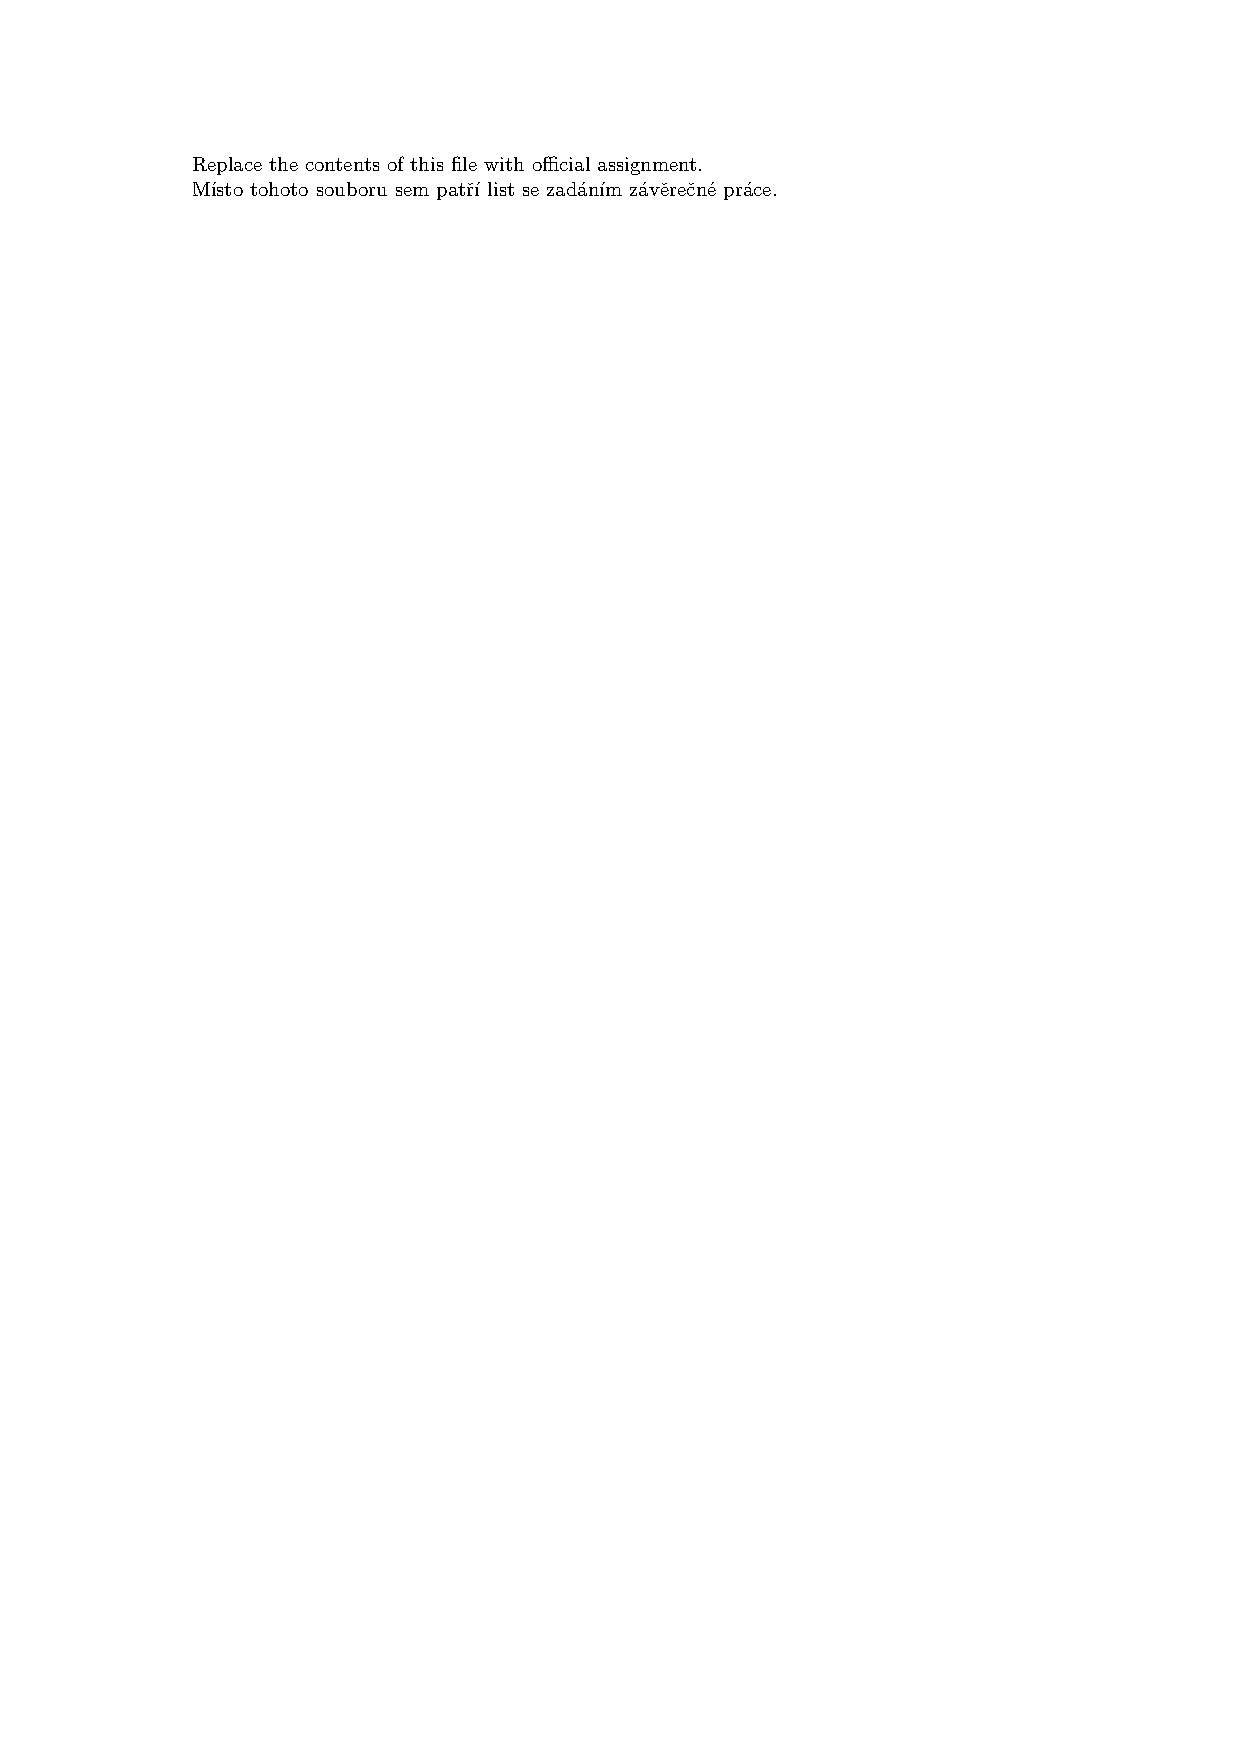
\includepdf[pages={1-}]{assignment-include.pdf} % replace that file with your thesis assignment provided by study office

\thispagestyle{empty}\cleardoublepage\maketitle % do not remove these three commands

\imprintpage % do not remove this command

\tableofcontents % do not remove this command
%%%%%%%%%%%%%%%%%%%%%%
% list of other contents: figures, tables, code listings, algorithms, etc.
% add/remove commands accordingly
%%%%%%%%%%%%%%%%%%%%%%
\listoffigures % list of figures
\begingroup
\let\clearpage\relax
\listoftables % list of tables
% \lstlistoflistings % list of source code listings generated by the listings package
% \listoflistings % list of source code listings generated by the minted package
\endgroup
%%%%%%%%%%%%%%%%%%%%%%
% list of other contents END
%%%%%%%%%%%%%%%%%%%%%%

%%%%%%%%%%%%%%%%%%%
% ACKNOWLEDGMENT
% FILL IN / MODIFY
% This is a place to thank people for helping you. It is common to thank your supervisor.
%%%%%%%%%%%%%%%%%%%
\begin{acknowledgmentpage}
    First and foremost, thanks to my parents, who have always supported me and
    enabled me to pursue my dreams, whatever they may be.

    I would also like to thank my supervisor, who spent an unbelievable amount
    of time and patience to break through my stubbornness and make this thesis
    what it is.

    Last but not least, thanks to my girlfriend, Jana. Without her support,
    this work would never have come to be.
\end{acknowledgmentpage} 
%%%%%%%%%%%%%%%%%%%
% ACKNOWLEDGMENT END
%%%%%%%%%%%%%%%%%%%


%%%%%%%%%%%%%%%%%%%
% DECLARATION
% FILL IN / MODIFY
%%%%%%%%%%%%%%%%%%%
% INSTRUCTIONS
% ENG: choose one of approved texts of the declaration. DO NOT CREATE YOUR OWN. Find the approved texts at https://courses.fit.cvut.cz/SFE/download/index.html#_documents (document Declaration for FT in English)
% CZE/SLO: Vyberte jedno z fakultou schvalenych prohlaseni. NEVKLADEJTE VLASTNI TEXT. Schvalena prohlaseni najdete zde: https://courses.fit.cvut.cz/SZZ/dokumenty/index.html#_dokumenty (prohlášení do ZP)
\begin{declarationpage}
I hereby declare that the presented thesis is my own work and that I have cited all
sources of information in accordance with the Guideline for adhering to ethical
principles when elaborating an academic final thesis.

I acknowledge that my thesis is subject to the rights and obligations stipulated by the
Act No. 121/2000 Coll., the Copyright Act, as amended. In accordance with Article 46(6)
of the Act, I hereby grant a nonexclusive authorization (license) to utilize this thesis,
including any and all computer programs incorporated therein or attached thereto and
all corresponding documentation (hereinafter collectively referred to as the “Work”), to
any and all persons that wish to utilize the Work. Such persons are entitled to use the
Work in any way (including for-profit purposes) that does not detract from its value.
This authorization is not limited in terms of time, location and quantity. However, all
persons that makes use of the above license shall be obliged to grant a license at least
in the same scope as defined above with respect to each and every work that is created
(wholly or in part) based on the Work, by modifying the Work, by combining the Work
with another work, by including the Work in a collection of works or by adapting the
Work (including translation), and at the same time make available the source code of
such work at least in a way and scope that are comparable to the way and scope in
which the source code of the Work is made available.
\end{declarationpage}
%%%%%%%%%%%%%%%%%%%
% DECLARATION END
%%%%%%%%%%%%%%%%%%%

\printabstractpage % do not remove this command


\mainmatter\mainmatterinit % do not remove these two commands

%%%%%%%%%%%%%%%%%%%
% THE THESIS
% MODIFY ANYTHING BELOW THIS LINE
%%%%%%%%%%%%%%%%%%%

\chapter{Introduction}
At the core of every computer program lies the Central Processing Unit (CPU),
which is responsible for executing programs. The CPU excels at performing very
primitive operations very fast. These operations, called instructions, perform
simple arithmetics, move values from and to memory, and change the control flow
of the program. They are encoded as a sequence of binary numbers, which are
easy for the CPU to understand, but are rather incomprehensible for humans.

To help programmers better understand written programs, a text mapping was
created called \textit{assembly language}. Each instruction is assigned a text
representation, as are the operands of the instruction. The control flow
instructions do not have to jump to an address offset but can instead use
labels. An example of a simple program in both an assembly language and a
machine code can be seen in figure~\ref{fig:simple-assembly}. If a programmer
is familiar with the instruction set architecture of the processor, they can
easily recognize the instructions the program is made of.

\begin{figure}
    \begin{subfigure}{1.0\textwidth}
        \begin{lstlisting}
01010101 01001000
10001001 11100101
10001001 01111101
11111100 10000011
01111101 11111100
00000000 01111110
00000111 10111000
00000001 00000000
00000000 00000000
11101011 00000101
10111000 00000000
00000000 00000000
00000000 01011101
11000011
        \end{lstlisting}
        \caption{A machine code program.}
        \label{subfig:machine-code}
    \end{subfigure}
    \begin{subfigure}{1.0\textwidth}
        \begin{lstlisting}
positive:
        push    rbp
        mov     rbp, rsp
        mov     -4[rbp], edi
        cmp     -4[rbp], 0
        jle     neg
        mov     eax, 1
        jmp     pos
neg:
        mov     eax, 0
pos:
        pop     rbp
        ret
        \end{lstlisting}
        \caption{An assembly program.}
        \label{subfig:assembly}
    \end{subfigure}\vspace{0.5cm}
    \begin{subfigure}{1.0\textwidth}
        \begin{minted}[]{c}
bool positive(int n) {
    if (n > 0) {
        return true;
    } else {
        return false;
    }
}
        \end{minted}
        \caption{A program in the C language.}
        \label{subfig:c}
    \end{subfigure}
    \vspace{0.5cm}
    \caption{An example of a program that checks if a number is positive, shown
    in an assembly language, in a machine code, and in the C programming
    language.}
    \label{fig:simple-assembly}
\end{figure}

However, as computers became increasingly more powerful, so did the programs
became bigger and more complex. When programming in the assembly language, the
programmer must have extensive knowledge of the processor's internal workings.

To spare the programmers from this, high-level programming languages were
created. These are designed to abstract from the specific machine the program
will run on, allowing programmers to focus more on their tasks. As shown in
figure~\ref{subfig:c}, even a simple program written in the C programming
language~\cite{krc}, one of the oldest programming languages around, provides a
clear understanding of the functionality. In contrast, examining the equivalent
program in assembly language, as seen in figure~\ref{subfig:assembly}, requires
knowledge of the specific architecture of the machine. High-level languages
also introduce control flow statements, which makes the code easier to follow
compared to assembly jumps~\cite{gotobad}.

But processors only understand machine code and high-level languages are far
from it. Therefore, a translation of a high-level language program into a
machine code program is necessary. This is a task for a \textit{compiler}. The
compiler is a program that reads source code of a high-level language and
produces machine code. Compilers are highly complex software; we will discuss
them in detail in chapter~\ref{section:source-level-debugging}. For now, it is
crucial to understand that the computer cannot directly run the source code of
a high-level language and that it is translated into machine code.
Additionally, compilers often take advantage of unique features of the
architecture to make the programs faster~\cite{dragon-book}.

\section{Debugging}
\begin{figure}
    \begin{minted}[
            linenos,
]{c}
int binary_search(int* arr, int len, int n) {
    int lo = 0;
    int hi = len;
    while (lo < hi) {
        int i = (lo + hi)/2;
        if (arr[i] < n) {
            lo = i;
        } else if (arr[i] > n) {
            hi = i;
        } else {
            return 1;
        }
    }
    return 0;
}
    \end{minted}
    \caption{A possible implementation of the binary search algorithm written
    in the C programming language.}
    \label{fig:binary-search}
\end{figure}

In figure \ref{fig:binary-search}, we present a more complicated example of a
program written in a high-level programming language. This is an implementation
of the binary search algorithm. As an input, it receives a sorted sequence of
numbers and a number $n$. The algorithm then checks whether the number $n$ is
in the sequence. This algorithm is widely used when searching in sorted
sequence because of its $\mathcal{O}(\text{log}_2(n))$
complexity~\cite{pruvodce}.

Programs are mostly written by humans, who tend to make
mistakes~\cite{human-error}. We are no exception, as we have also made a
mistake in the binary search program. Let us try to run the program with a
\texttt{[1,2,3]} sequence and search for the number $4$. This number is not in
the sequence, so the expected output would be $0$. Instead, if we ran the
program, it would run forever because of a mistake we made in the source code.
Such mistakes are called \textit{bugs}\footnote{The term \textit{bug} actually
comes from an actual bug that got stuck in relays back when computers were made
from relays. They literally had to debug the machine by taking the bug out.}.
The process of finding these mistakes and correcting them is called
\textit{debugging}~\cite{art-of-testing}.

There are several approaches to debugging. We could try to look at the source
code and find the mistake this way\footnote{Do note that this approach does not
scale well with bigger programs.}. Here we could assume that the condition
\texttt{lo < hi} never comes to be since it is the most obvious place where we
could get stuck forever. Now, it would be helpful if we could see the states of
\texttt{lo} and \texttt{hi} in each iteration of the cycle. We could resort to
print statements, but that is not very flexible. If we changed our minds and
wanted to also see the value of variable \texttt{i}, we would have to recompile
the program and rerun it. The output can also quickly get overwhelming,
especially in an infinite loop. A different approach is to use a debugger, which
is a special tool fitted exactly for this purpose.

Debugger is able to inspect the state of another program, like the values of
its variables. It is also able to control the flow of the program. They allow
\textit{breakpoints} to be set at each line of the source
code\footnote{Advanced debuggers allow breakpoints to be set inside
expressions. This is especially important for functional languages, as their
functions often consist of one big expression.}. When the program is about to
execute the line of code with the breakpoint, the control is passed back to the
debugger, and the user can inspect the state of the program at that line. There
are also conditional breakpoints, which only trigger when some condition holds.
An example of such a condition can be that the breakpoint gets activated only
when \texttt{i == 3}.

Finally, debuggers also allow \textit{stepping}. There are several kinds of
steps:
\begin{itemize}
    \item \textit{step-in} - Executes the current statement and stops on the
        next one. If the current statement is a function call, it will be
        executed, and the program will be paused on the first statement in that
        function.
    \item \textit{step-over} - Same as a step-in, but if the current statement
        is a function call, the program will be paused on the next statement
        after the call.
    \item \textit{step-out} - Executes as much as needed to return from the
        current function. Stops on the next statement that should be executed
        after the function returns.
\end{itemize}

To illustrate the workings of the debugger, let us look back at the program in
figure~\ref{fig:binary-search}. We will place a breakpoint on line $6$ after
$i$ is set and we will monitor how the values in variables \texttt{lo} and
\texttt{hi} change. If the program is run with the debugger attached, an output
similar to what is displayed in figure~\ref{fig:lldb-debug1} will be seen.
Here, it is possible to see the line on which the execution was stopped. It is
also possible to print the state of variables. In each loop, we could print the
value of a variable and then continue execution until another breakpoint is
hit. If we continue, the execution will again be stopped on line $6$. The value
of \texttt{hi} will not change, which is expected. Variable \texttt{lo} will
gain the following values: $0, 1, 2, 2, 2, \dots$ It apparently gets stuck at
$2$. The value of variable $i$ is computed as $i = (\text{lo} + \text{hi})/2 =
(2 + 3)/2 = 2$, because division in C rounds the value down. The fix is to
change the line $7$ to \texttt{lo = i + 1}. With the debugger, it was simple to
find out where the error came from, and we did not have to recompile the
program.

\begin{figure}
\begin{minted}{c}
   3   	    int hi = len;
   4   	    while (lo < hi) {
   5   	        int i = (lo + hi)/2;
-> 6   	        if (arr[i] < n) {
   7   	            lo = i;
   8   	        } else if (arr[i] > n) {
   9   	            hi = i;
Target 0: (a.out) stopped.
> p lo
(int) $0 = 0
> p hi
(int) $1 = 3
\end{minted}
    \caption{Debugging session in the LLDB~\cite{lldb} debugger, showing
    breakpoint hit report and printing variable values.}
    \label{fig:lldb-debug1}
\end{figure}

We previously mentioned that processors themselves only understand machine
code. Hence, the question arises as to how the debugger can know about lines,
variables, and similar traits of the source code when the program itself is
just machine code. The compiler has to lend a hand here. It embeds information
about the source code, either into the executable itself or into a separate
file. For example, it maps lines of source code to machine code instructions.
Thanks to this mapping, the debugger knows that line $x$ corresponds to
instruction $y$ in the machine code and can put a breakpoint there. If the
compiler does not emit any information into the executable, the debugger would
only work with assembly, as seen in figure~\ref{fig:lldb-debug2}. This can be
very difficult for the programmer to work with compared to debugging the source
code directly.

\begin{figure}
\begin{lstlisting}
->  0x100003e3c <+112>: b      0x100003e78               ; <+172>
    0x100003e40 <+116>: ldr    x8, [sp, #0x20]
    0x100003e44 <+120>: ldrsw  x9, [sp, #0xc]
    0x100003e48 <+124>: ldr    w8, [x8, x9, lsl #2]
\end{lstlisting}
\caption{Example of debugging a program in the LLDB debugger without debugging
    information generated by the compiler.}
\label{fig:lldb-debug2}
\end{figure}

\section{Teaching Compilers}
Many schools about computer science have a compiler course, and the Faculty of
Information Technology, CTU, is no exception. The course is called \textit{Code
Generators} (NI-GEN). In this course, students are tasked to build a simple
compiler from a C-like language called TinyC. The target of the compiler is the
Tiny x86 (T86) architecture. This architecture does not have a processor that
implements it. Instead, a virtual machine, a program that reads the assembly
and executes it, was created for it. The architecture is supposed to ease the
code generation and let the students focus on the more interesting parts of the
compiler, like register allocation or optimization, instead of the
uninteresting details of real CPU architectures.

There is, however, a problem with using T86, as it has almost non-existing
debugging support. So if a compiler of some student generates the code badly,
which is frankly inevitable, it takes a non-trivial amount of effort to find
the error. T86 has some very light debugging capability, but it is far from
real debugging. Also, compiling debugging information is not taught in the
NI-GEN course because there is no reason to as of now. If a debugger was
provided to the students, it might be incentivizing to compile such information
to ease their lives later when they need to find errors in their compilers.
This way, they will also learn how and what information the compiler needs to
embed for the debugger to work.

\section{Goals of the Thesis}
The primary goal is to add debugging support to the T86 and create a debugger
that supports debugging both on the machine and source code levels. The
debugger should be extensible enough to also work with an intermediate
representation. The debugger should be similar to real-world debuggers in terms
of how it works. This will require non-trivial changes in the T86 virtual
machine source code. The students' compilers will also have to generate
debugging information. The format of the debugging information should be so
that it is not discouraging for students to generate but also comparable to
debugging information generated by real compilers.

\section{Structure of the Thesis}
\begin{enumerate}
    \item The \textit{Introduction} is the motivation behind the thesis and
        introduces basic terms with which should the reader be familiar.
    \item \textit{Debugging Techniques} describes how are debuggers implemented
        and what support is required on various levels (OS, processors,
        compilers) to make their implementation possible.
    \item \textit{Tiny x86} describes the T86 architecture and discusses some
        of the parts of the virtual machine, mainly its existing debugging
        capabilities.
    \item \textit{Implementation} focuses on extending the T86 instruction set
        and adding a debugging interface to the virtual machine. It also
        describes the implementation of the debugger and the chosen format of
        the debugging information.
    \item \textit{Evaluation} evaluates the performance of the debugger and its
        ease of use.
    \item \textit{Conclusions} summarizes the result of the thesis and speaks
        of possible future work.
\end{enumerate}

\chapter{Debugging Techniques}

\begin{quote}
  \textit{Debugging is twice as hard as writing the code in the first place.
    Therefore, if you write the code as cleverly as possible, you are, by
    definition, not smart enough to debug it.}\begin{flushright}
    \scriptsize{Brian W. Kernighan}
  \end{flushright}
\end{quote}

We need the compiler to emit debugging information to debug a program written
in a high-level programming language. Without this information, we can debug
the program at the assembly level. This can still be useful, for example, for
reverse engineering. Furthermore, without assembly-level debugging, there is no
source-level debugging since it builds upon it. This chapter describes at which
level and what kind of debugging support is provided. First, we will mention
what kind of mechanism the CPU itself offers. Going one step higher, we will
talk about the API that various operating systems provide. Finally, we will
discuss how compilers and debuggers can allow us to debug source code, although
the program we debug was compiled into a machine code program.

\section{CPU Level Support}\label{section:cpu-debug-support}
The CPU can only execute machine code which is made of instructions. It also
has several registers to help with computations. Which instructions and
registers the CPU has can differ from CPU to CPU. This is specified by an
\textit{Instruction Set Architecture} (ISA)~\cite{isa}. It is an abstract
interface between the hardware and the lowest-level software (machine code). It
contains all information needed to write a program in machine code. In general,
ISA specifies the following: 
\begin{itemize}
    \item Set of machine code instructions - Specifies instructions the ISA has
        and what operands each instruction has.
    \item Register set - Which registers the ISA has\footnote{Strictly speaking
        ISA doesn't have to use registers. It's possible to use only stack or
        accumulator, but most used ISAs use registers, so we'll ignore those
        architectures. }.   
    \item Addressing modes - Possible methods to refer to memory or register. 
\end{itemize}
This list is not exhaustive, but for our purposes, it suffices. For each
instruction and operand, it is specified how they should be encoded into
binary. CPU then \textit{implements} some ISA. If two different CPUs implement
the same ISA, then they should be able to run the same machine code program.
For example, personal computers often use the x86-64 while mobile devices like
smartphones or tablets use the ARM architecture~\cite{riscvscisc2}. The ARM
architecture is also beginning to find its way into the computer space. For
example, Apple Silicon uses ARM architecture.

The x86-64 architecture is so called \textit{Complex Instruction Set
Architecture} (CISC). The CISC instructions often perform many actions at once,
have varying lengths, and take multiple clock cycles to
complete~\cite{intel-manual}. On the other hand, the ARM architecture is
\textit{Reduced Instruction Set Architecture} (RISC). The number of
instructions is smaller. They are intended to be small building blocks from
which complex operations may be created by using many of them. Each instruction
in RISC also has the same length. Both architectures have their pros and cons,
although some literature suggests that in modern days the choice of
architecture is irrelevant if one is only considering performance and power
consumption~\cite{riscvscisc1, riscvscisc2}. Unless specified otherwise, the
rest of this chapter will be talking about x86-64. This is because the T86
architecture, described in section ~\ref{section:T86}, is loosely based on
x86-64, so it is most relevant for us.

In the first chapter, we briefly mentioned that machine code programs can be
written in assembly language instead. Assembly is almost a one-to-one mapping
to machine code. When showing programs, we will show them in assembly so that
they are readable. In figure~\ref{fig:assembly-example2}, we present another
example of a program written in the C programming language that was compiled
into an assembly for the x86-64 architecture. As seen, instructions have
various operands. Most often registers (\texttt{rbp, rsp, eax}), memory
(\texttt{[rbp-4]}), or labels (like \texttt{L2}). Labels are not part of
machine code; instead, a memory address has to be provided. This is a small
part where assembly and machine code differ. For a detailed overview of the
x86-64 instruction set, see~\cite{intel-manual}.

\begin{figure}
    \begin{lstlisting}
max:
    push    rbp
    mov     rbp, rsp
    mov     QWORD PTR [rbp-24], rdi
    mov     DWORD PTR [rbp-28], esi
    mov     rax, QWORD PTR [rbp-24]
    mov     eax, DWORD PTR [rax]
    mov     DWORD PTR [rbp-4], eax
    mov     DWORD PTR [rbp-8], 1
    jmp     .L2
.L3:
    mov     eax, DWORD PTR [rbp-8]
    cdqe
    lea     rdx, [0+rax*4]
    mov     rax, QWORD PTR [rbp-24]
    add     rax, rdx
    mov     eax, DWORD PTR [rax]
    cmp     DWORD PTR [rbp-4], eax
    cmovge  eax, DWORD PTR [rbp-4]
    mov     DWORD PTR [rbp-4], eax
    add     DWORD PTR [rbp-8], 1
.L2:
    mov     eax, DWORD PTR [rbp-8]
    cmp     eax, DWORD PTR [rbp-28]
    jl      .L3
    mov     eax, DWORD PTR [rbp-4]
    pop     rbp
    ret
    \end{lstlisting}
    \caption{An example of an assembly program that was compiled from a program
    written in the C programming language using the GCC compiler.}
    \label{fig:assembly-example2}
\end{figure}

\subsection*{Registers}\label{subsection:registers}

The x86-64 architecture has a set of general purpose registers.
Some of these are
\begin{itemize}
    \item \texttt{rax} - Accumulator for operands and results data,
    \item \texttt{rcx} - Counter for string and loop operations,
    \item \texttt{rsp} - Stack pointer,
    \item \texttt{rbp} - Pointer to data on the stack.
\end{itemize}
Although there is a special role for each register, it is more of a convention
for some. It is not necessary to use the \texttt{rcx} register exclusively for
loop operations. Although the \texttt{rsp} and \texttt{rbp} are called general
purpose, they are often only used for pointing at the top of the stack,
respectively to the base of the stack. Stack is a special part of program
memory with LIFO semantics. It can be used to store the intermediate result,
arguments to functions, return address, etc. The \texttt{rbp} register is weird
one because it has this very special purpose but is still considered part of
the general purpose registers~\cite{intel-manual}. One might use it for storing
calculations, but it would make the rest of the instructions that work with
stack behave unexpectedly.

The instruction pointer register (\texttt{rip}) contains the address of the
current instruction to be executed. Programs are executed sequentially from top
to bottom, with particular instructions having the ability to change the
control flow. When an instruction gets executed, the size of the instruction
will be added to the value in the \texttt{rip} register. This will advance the
instruction pointer to the next instruction. Alternatively, if the instruction
changes the control flow, the value in the instruction pointer will be changed
to the instruction's destination. The register can also be changed directly.

Another interesting register is the \texttt{eflags} register. The register is
made up of various flags, which can alter the CPU behavior, or the CPU itself
sets them as a result of some instruction. For example, the instruction
\texttt{cmp} compares its two operands, and if they are the same, the
\textit{zero} flag in the \texttt{eflags} register will be set.

\subsection{Interrupts}\label{section:interrupts}
An interrupt is a special request to the CPU to stop the execution of the
current program and to quickly react to the reason that caused the
request~\cite{computer-architecture}. An example of such event can be a
keyboard press or an error in a program (division by zero). There are two main
categories~\cite{intel-manual}
\begin{itemize}
    \item An \textbf{interrupt} is an asynchronous\footnote{Meaning that the
        interrupt may happen when another instruction is being processed (not
        on the CPU clock edge).} event that is typically triggered by an
        Input/Output (IO) device.
    \item An \textbf{exception} is a synchronous event that is
        generated when the processor detects one or more predefined conditions
        when executing an instruction. These are further divided into three
        classes: faults, traps, and aborts.
\end{itemize}


For the rest of this thesis, we will use the word interrupt interchangeably for
both interrupt and exception, although we will mainly talk about exceptions.
This is to disambiguate the exceptions at a programming language level (like
C++) and Microsoft structured exceptions, which are the subject of
section~\ref{section:seh}. When an interrupt or exception happens, the
processor halts the execution of a current program and switches to a specific
interrupt handler. An interrupt handler is just a sequence of instructions that
gets executed when the interrupt happens. 

An example of an exception is the \texttt{int3} instruction. When this
instruction is executed, an interrupt is generated. This instruction is
specifically meant to be used as a breakpoint. In theory, we could supply code
that will be responsible for handling the breakpoint as the interrupt handler.
We could then set the \texttt{int3} instruction where we want the breakpoint to
occur and inspect the code through the interrupt handler. However, on modern
PCs, an Operating System (OS) governs the PC and consequently is responsible
for setting interrupt handlers. Alas, we cannot touch the interrupt handler
directly. Instead, the OS will have to provide another layer of support for
debugging.

Recall the EFLAGS register mentioned in section~\ref{subsection:registers}.
There is a special flag called the trap flag. When it is set, the CPU will
issue an interrupt after every executed instruction. This could be useful if we
wanted to inspect execution instruction by instruction.

% Page ~3644 in intel manual
The CPU may also contain special debug registers. The x86-64 architecture has
six of them, named \texttt{dr0} to \texttt{dr7}, with \texttt{dr4} and
\texttt{dr5} being synonyms for \texttt{dr6} and \texttt{dr7} on most CPUs,
otherwise, they are reserved anyway and cannot be used. The CPU provides
special breakpoints through these registers. Each of the first four registers
contains an address of the breakpoint. The debug status register \texttt{dr6}
contains debug conditions that were sampled at last debug interrupt. Lastly,
the debug control register \texttt{dr7} is used to enable and disable
breakpoints for each of the address registers and set breakpoint conditions.
The conditions are either instruction execution on a specific address or a
memory read or write. When the breakpoints are hit, for example, the address
stored in \texttt{dr0} is written into, the breakpoint is enabled, and the
condition is set to memory write in the \texttt{dr7} register, an interrupt is
issued by the CPU and the \texttt{dr6} register contains information about
which register caused the interrupt~\cite{intel-manual}.

\subsection{Superscalar CPUs}\label{section:superscalar-cpu}
Modern CPUs do not execute instructions strictly one by one. They instead use
\textit{pipelines} and \textit{out-of-order execution}~\cite{isa,
computer-architecture}. This means that they can execute several instructions
at once and can execute them in non-sequential order. The observable behavior
of the program has to be the same as if it was run sequentially. The CPU has to
be careful about which instruction it can run in parallel and out of order. The
execution of an instruction consists of several stages, which together form an
\textit{execution pipeline}. The stages can be \textit{Fetch}, \textit{Decode},
\textit{Execute}, \textit{Memory}, and \textit{Writeback}; this may vary
depending on the architecture. However, the general ideas behind it are the
same. The instruction must pass all these stages to be successfully executed.
To maximize efficiency, all stages are occupied by an instruction. This means
that when instruction $x$ leaves the fetch stage, it goes to the decode stage,
and instruction $y$ is put into the fetch stage.

However, when the next instruction is a conditional jump, there may be no way
to be sure if the jump will be taken. CPUs deal with it in various ways and try
to predict the right branch. Sometimes, however, the prediction fails, and the
whole pipeline needs to be flushed. The same action must be taken when an
interrupt occurs. The execution changes to the interrupt handler, and the
pipeline must therefore be flushed because it contains instructions from the
previous location before the control flow was switched to the handler. Also, if
we hit the breakpoint, we want to make sure that instructions before it were
all executed and that none were executed after. Otherwise, it would be very
confusing for the user that tries to debug the program.

\section{Operating System Support}
Operating system is a layer between computer components (CPU, memory,
input/output devices, \dots) and software. It is responsible for handling all
the resources so programmers do not have to think about it~\cite{modern-os,
os-concepts}. Managing resources is not only to make writing programs easier
but to make sure that the programs are safe from each other. Modern operating
system allows to run multiple programs at once (or at least offer the illusion
that it can) and they make sure that one program cannot overwrite data or
otherwise interfere with other programs. Normal programs run in so-called
\textit{user space}, which has limited capabilities. The kernel on the other
hand runs in \textit{kernel space}. It has full access to the hardware of the
computer, can use all instructions, can permit or mask interrupts, and so on.

However, if programs were kept to user space all the time they would be very
limited. Sometimes, they need to escape the confinement of the OS, for example,
to read a file or communicate with other processes. Operating systems provide
an interface through which the user space program can leverage a small part of
the kernel in form of system calls. They offer a way of requiring some service
from the OS. This API is often in form of C and C++
functions~\cite{os-concepts}. A part of these functions is a special
instruction, like \texttt{SYSCALL} on x86-64~\cite{intel-manual}, that switches
the mode to kernel space.

The most used operating systems today are Microsoft Windows, Linux, and MacOS.
Linux and MacOS systems are somewhat similar, but Windows is very different. To
debug programs, we need to be able to read and modify the state of a running
program. This is in direct conflict with the encapsulation the operating system
is trying to achieve. As such, the operating system must provide an API through
which we can do these operations that are needed for debugging.

\subsection{Linux}\label{section:linux-dbg}
Linux offers a special system call which is very handy for debugging. It is
called \texttt{ptrace}~\cite{ptrace} - process trace. It has the following
signature: \texttt{ptrace(request, PID, void* addr, void* data)}. The request
is a \texttt{PTRACE\_COMMAND}, which specifies the behavior of the function
(for example \texttt{PTRACE\_SINGLESTEP}), process id (PID) of some process
(presumably the debuggee) and two other parameters, whose meaning change
depending on the \texttt{PTRACE\_COMMAND} that was chosen\footnote{Peak API
design!}. It allows one to observe and control the execution of another
process; this process will be the debuggee. In the context of this chapter, we
will sometimes use the word tracee for the debuggee, and tracer for the
debugger, to be consistent with ptrace documentation.

The \texttt{ptrace} function has many commands, here are some of the most important:
\begin{itemize}
    \item \texttt{PTRACE\_PEEKTEXT, PTRACE\_PEEKDATA} - Read tracee's memory.
    \item \texttt{PTRACE\_POKETEXT, PTRACE\_POKEDATA} - Write into tracee's
          memory.
    \item \texttt{PTRACE\_GETREGS} - Read tracee's register values.
    \item \texttt{PTRACE\_SETREGSET} - Modify tracee's register values.
    \item \texttt{PTRACE\_GETSIGINFO} - Retrieve information about the signal
                                        that caused tracee to stop.
    \item \texttt{PTRACE\_CONT} - Restart the stopped tracee process.
    \item \texttt{PTRACE\_SINGLESTEP} - Restart the stopped tracee but
          stop it after executing one instruction.
\end{itemize}

Linux, however, needs some way of notifying the debugger that the tracee
encountered a breakpoint or that some other event requiring debugger attention
happened. To this end, \textit{signals} are used. They serve as an abstraction
on top of the CPU interrupts. Interrupts are sent by the CPU and processed by
the operating system kernel. Signals are sent by the operating system kernel
and received by processes. They can also be sent by a process, that however
happens via system calls and the kernel is the one who sends the signal, so the
statement still stands.

A signal is used in UNIX and Linux systems to notify a process that a
particular event has occurred~\cite{os-concepts}. When a process receives a
signal, it stops its execution and starts the execution of a signal handler.
There are various signal types. Most signals can have a custom signal handler
defined by the process. If no handler is defined, then the OS provides a
default one. However, handlers for \texttt{SIGKILL} and \texttt{SIGSTOP} cannot
be changed~\cite{signals}.

The reason for sending a signal to a process can, for example, be a CPU
interrupt (like division by zero or breakpoint hit) or a system call
(\texttt{kill(pid, signal)}). One such signal is the \texttt{SIGTERM}, which
can be sent to a process to "ask it" to exit. The process can handle this
request, for example, to save some state before exiting. It can also be
entirely ignored. To prevent this, a signal \texttt{SIGKILL} can be used, which
cannot be handled, ignored, or blocked.

To begin tracing a command \texttt{PTRACE\_ATTACH} may be used for an already
existing process, or a \texttt{fork} followed with a child calling
\texttt{PTRACE\_TRACEME} and typically \texttt{execve}. When the tracee is
being traced, it will stop each time a signal is delivered to it, even if it
chooses to ignore said signal. The tracer will be notified that the tracee
received a signal at its next call to the \texttt{waitpid} function. When the
tracee is stopped, the tracer can initiate various ptrace requests listed above
to inspect and change the state of the tracee~\cite{ptrace}.

In chapter \ref{section:interrupts}, we mentioned that the debug instructions
cause an interrupt. The Linux kernel, however, does not permit us to work with
interrupt handlers. Instead, it translates those interrupts into signals. So
when the tracee executes the \texttt{int3} instruction, it will receive a
signal that we will catch with the \texttt{waitpid} function.

\subsubsection{Debugger implementation}
Now, we have all the necessary building blocks to build a simple debugger on
the Linux operating system running on the x86-64 platform. Running a program
under the debugger is simple. Figure~\ref{fig:debugger-init} shows the
initialization of the debugger. It uses the fork-exec idiom. The \texttt{fork}
system call creates an exact copy of the process as a child except the
following: process ID (PID) of the child is different. In the parent process,
\texttt{fork} returns the PID of the child. In the child, $0$ is returned. The
child initiates the \texttt{PTRACE\_TRACEME} call, which indicates that this
process is to be traced by its parent. Then it calls the \texttt{execve} system
call, which replaces this program with the one we want to debug. The execve
causes a \texttt{SIGTRAP} signal on completion because the process is being
traced~\cite{execve}.

The parent first issues a \texttt{waitpid} system call. This waits for the
child \texttt{execve} to finish. The debugger then has a chance to debug the
child immediately because it is stopped. The \texttt{while} loop can then
request input from the user and act accordingly. The tracee can be continued by
\texttt{PTRACE\_CONT} command.

\begin{figure}
    \begin{minted}{c}
pid_t pid = fork();
if (pid == 0) {
    // Begin tracing
    ptrace(PTRACE_TRACEME, 0, NULL, NULL);
    // Replace the code with the intended tracee code
    execve(executable, argv, NULL);
} else {
    int w;
    waitpid(pid, &w, 0);
    while(...) {
        // Main debugger loop
    }
}
    \end{minted}
    \caption{Linux debugger implementation - Initialization of the debuggee
    process.}
    \label{fig:debugger-init}
\end{figure}

Reading and writing to memory is simple. The \texttt{PTRACE\_PEEKTEXT} and
\texttt{PTRACE\_POKETEXT} are used for this purpose. This call reads or writes
a word (32 or 64 bits, depending on the Linux variant) into the tracee's
memory. However, if we want to write an arbitrary amount of bytes, we have to
work around the word limitation. We need to write by blocks, and for the last
one, we have to pad the write with already existing data if the block size does
not divide the word size. Figure~\ref{fig:write-read} shows how to read and
write precisely one byte of memory at a given address, which is simpler to
implement but not ideal for writing many bytes.

\begin{figure}
    \begin{minted}{c}
uint8_t read_memory(pid_t pid, uint64_t address) {
    uint64_t data = ptrace(PTRACE_PEEKDATA, pid, address, NULL);
    return (uint8_t)data;
}

void write_memory(pid_t pid, uint64_t address, uint8_t data) {
    uint64_t old = ptrace(PTRACE_PEEKDATA, pid, address, NULL);
    uint64_t new_data = (old & ~0xFF) | data;
    ptrace(PTRACE_POKEDATA, pid, address, new_data);
}
    \end{minted}
    \caption{Reading and writing one byte to debuggee memory using ptrace.}
    \label{fig:write-read}
\end{figure}

Registers are similar to a memory in regards to how to read them. Linux
contains a predefined structure \texttt{user\_regs\_struct}, which maps all
registers on the current architecture. The command \texttt{PTRACE\_GETREGS}
then fills up this structure with the value in registers. To save registers,
\texttt{PTRACE\_SETREGS} can be used. One has to pass the whole structure, so
if we want to modify only some registers, we first need to fetch the structure,
fill the registers we want with values, and then finally use \texttt{SETREGS}.
An implementation can be seen in figure~\ref{fig:set-register}, the
\texttt{get\_register} functions maps the structure members to the register's
name. Since the address of the current instruction to be executed is also
stored in a register (\texttt{rsp}), we now have access to it.

\begin{figure}
    \begin{minted}{c}
void set_register(pid_t pid, const char* name, uint64_t data) {
    struct user_regs_struct regs;
    ptrace(PTRACE_GETREGS, pid, NULL, &regs);
    uint64_t* reg_data = get_register(&regs, name);
    *reg_data = data;
    ptrace(PTRACE_SETREGS, pid, NULL, &regs);
}
    \end{minted}
    \caption{Setting debuggee register value using ptrace.}
    \label{fig:set-register}
\end{figure}

Breakpoints are more interesting. Debuggers often allow to enable and disable a
breakpoint, so we will distinguish between setting a breakpoint and enabling
it. Setting a breakpoint just means that the debugger needs to keep track of
where the breakpoint was set and if it is enabled or disabled. Enabling a
breakpoint means writing into the program memory the debug instruction (we will
use the x86-64 \texttt{int3} instruction with opcode \texttt{0xCC}). Figure
\ref{fig:with-and-without-bp} shows how code looks with and without enabled
breakpoint. The blue color shows the new breakpoint. On line $2$, the opcode
changes from \texttt{0x83} to \texttt{0xCC}. Since the breakpoint is set via
the \texttt{PTRACE\_POKEDATA}, which only works data blocks, one has to pad the
breakpoint opcode with already existing data, those are marked by the red
color. Also, the rewritten data (in this case the \texttt{0x88} has to be kept
so that the breakpoint may later be deactivated. Abbreviated implementation can
be found on \ref{fig:breakpoint-enable}.

\begin{figure}
    \begin{minipage}{0.45\textwidth}
        \begin{Verbatim}
  01 d0     add eax,edx
  88 45 fd  mov [rbp-0x3],al
  ff e0     jmp rax
        \end{Verbatim}
    \end{minipage}
    \hfill\vline\hfill
    \begin{minipage}{0.45\textwidth}
        \begin{Verbatim}[commandchars=\\\{\}]
  01 d0     add eax,edx
  \textcolor{blue}{cc} \textcolor{red}{45} \textcolor{red}{fd}  \textcolor{blue}{int3}
  ff e0     jmp rax
        \end{Verbatim}
    \end{minipage}
    \caption{Code with and without a breakpoint. The breakpoint is highlighted
    by the blue color. The red color shows invalid instruction.} 
    \label{fig:with-and-without-bp}
\end{figure}

\begin{figure}
    \begin{minted}{c}
void enable(pid_t pid, struct breakpoint* bp) {
    if (bp->enabled) {
        return;
    }
    bp->backup = read_memory(pid, bp->address);
    write_memory(pid, bp->address, BP_OPCODE);
    bp->enabled = true;
}

void disable(pid_t pid, struct breakpoint* bp) {
    if (!bp->enabled) {
        return;
    }
    write_memory(pid, bp->address, bp->backup);
    bp->enabled = false;
}
    \end{minted}
    \caption{Enabling breakpoints, abbr.}
    \label{fig:breakpoint-enable}
\end{figure}

When a breakpoint is hit, the control is passed to the debugger. At this point,
the instruction pointer would point to the next instruction, which has opcode
\texttt{0x7D}, not \texttt{0xFF} (the \texttt{jmp} instruction) as might be
expected. This is because \texttt{int3} is an instruction with size $1$. It
gets executed, the instruction pointer is advanced by the size ($1$), and an
interrupt is issued. However, after the \texttt{int3}, there were operands to
the \texttt{mov} instruction (the red text in the figure). We definitely do not
want to interpret them as instruction. We found out that on some architectures,
advancing PC does not happen when an instruction that issues an interrupt is
executed, such as the ARM \texttt{BKPT} instruction. This was later confirmed
by looking at the LLDB code (under \verb|NativeProcessProtocol.cpp|), as it
only moves back the program counter for a few architectures.

Additionally, if we just moved back and resumed the program, we would again hit
the breakpoint, which is still set. We need to temporarily unset it, move one
instruction forward and set it again. The general idea behind it can be found
in figure~\ref{fig:continue}. With breakpoints, we essentially gained the
ability to single step as well.

\begin{figure}
    \centering
    \begin{tikzpicture}[
dot/.style = {circle, fill, minimum size=#1,
              inner sep=0pt, outer sep=0pt},
dot/.default = 0pt,
node distance = 0pt,
square/.style = {draw=black!60, fill=white!5, very thick, 
                 minimum height=1.2cm,
                 align=center,
                 text width=1.0cm,
                 outer sep=0pt,
                 trapezium stretches=true}, % To make all nodes of the same height
]
        \node (pro21) [square] {\texttt{0x01 add}};
        \node (pro31) [square,
                      right=of pro21] {\texttt{0xd0}};
        \node (pro41) [square, right=of pro31] {\texttt{0xcc int3}};
        \node (pro51) [square, right=of pro41] {\texttt{0x45}};
        \node (pro61) [square, right=of pro51] {\texttt{0xfd}};
        \node (pro71) [square, right=of pro61] {\texttt{0xff jmp}};
        \node (pro81) [square, right=of pro71] {\texttt{0xe0}};
        \node (text1) [text width=5cm,
                       right=0.1cm of pro81,align=justify]
                       {Just before hitting a breakpoint.};
        \node (ip1)   [dot, above=0.65cm of pro41] {};
        \draw[->] (ip1) -- (pro41);
        % second row
        \node (pro22) [square,
                      below=1cm of pro21] {\texttt{0x01 add}};
        \node (pro32) [square,
                      right=of pro22] {\texttt{0xd0}};
        \node (pro42) [square, right=of pro32] {\texttt{0xcc int3}};
        \node (pro52) [square, right=of pro42] {\texttt{0x45}};
        \node (pro62) [square, right=of pro52] {\texttt{0xfd}};
        \node (pro72) [square, right=of pro62] {\texttt{0xff jmp}};
        \node (pro82) [square, right=of pro72] {\texttt{0xe0}};
        \node (text2) [text width=5cm,
                       right=0.1cm of pro82,align=justify]
                       {After software breakpoint is executed.};
        \node (ip2)   [dot, above=0.65cm of pro52] {};
        \draw[->] (ip2) -- (pro52);
        % third row
        \node (pro23) [square,
                      below=1cm of pro22] {\texttt{0x01 add}};
        \node (pro33) [square,
                      right=of pro23] {\texttt{0xd0}};
        \node (pro43) [square, right=of pro33] {\texttt{0x88 mov}};
        \node (pro53) [square, right=of pro43] {\texttt{0x45}};
        \node (pro63) [square, right=of pro53] {\texttt{0xfd}};
        \node (pro73) [square, right=of pro63] {\textcolor{red}{\texttt{0xcc int3}}};
        \node (pro83) [square, right=of pro73] {\texttt{0xe0}};
        \node (text3) [text width=5cm,
                       right=0.1cm of pro83,align=justify]
                       {Move instruction pointer back,
                       replace the \texttt{int3} instruction
                       with the original one and set a breakpoint
                       at the next instruction.};
        \node (ip3)   [dot, above=0.65cm of pro43] {};
        \draw[->] (ip3) -- (pro43);
        % fourth row
        \node (pro24) [square,
                      below=1cm of pro23] {\texttt{0x01 add}};
        \node (pro34) [square,
                      right=of pro24] {\texttt{0xd0}};
        \node (pro44) [square, right=of pro34] {\texttt{0xcc int3}};
        \node (pro54) [square, right=of pro44] {\texttt{0x45}};
        \node (pro64) [square, right=of pro54] {\texttt{0xfd}};
        \node (pro74) [square, right=of pro64] {\texttt{0xff jmp}};
        \node (pro84) [square, right=of pro74] {\texttt{0xe0}};
        \node (text4) [text width=5cm,
                       right=0.1cm of pro84,align=justify]
                       {Resume the execution, remove the newly set breakpoint
                       and restore the old one.};
        \node (ip4)   [dot, above=0.65cm of pro74] {};
        \draw[->] (ip4) -- (pro74);
    \end{tikzpicture}
    \caption{A diagram of how a continue operation might be performed. The
    arrow signalizes an instruction pointer.}
    \label{fig:continue}
\end{figure}

However, putting a breakpoint on the instruction that will be executed next is
more challenging than it might appear. Due to the varying sizes of instructions
on CISC architectures, even determining the instruction that follows the
current one in the code is challenging. RISC architectures facilitate this
because all instructions have the same length. Finding the next instruction to
be executed may still pose a challenge if the instruction is a conditional
jump. Accurately determining where the jump will go can be an arduous task. To
achieve this, some debuggers use instruction emulators. Fortunately, some
architectures have built-in hardware support for single stepping, like the trap
flag we mentioned in section~\ref{section:cpu-debug-support}.

The ptrace library contains a special \texttt{PTRACE\_SINGLESTEP} command,
which executes one instruction in the tracee before sending the
\texttt{SIGTRAP} signal. The Linux kernel (as of v6.1.8) uses the previously
mentioned trap flag for x86-64~\cite{linuxkernel-trapflag}. The call will
return an error if the architecture does not provide a hardware-supported
single stepping. In lieu of the breakpoint dance mentioned earlier, the
singlestep command will be used in our implementation because x86-64 supports
it. Implementation is described in figure~\ref{fig:singlestep}. We presume that
the instruction pointer was moved when the breakpoint was hit, eliminating the
need to return one byte backward. This is more reasonable anyway, since we want
to show the user at which address the breakpoint hit happened. The
LLDB~\cite{lldb} debugger uses hardware support if there is one, else it uses
an instruction emulator. For instance, for the ARM architecture, LLDB uses an
instruction emulator, whereas, for the x86-64, it uses the trap flag.

\begin{figure}
    \begin{minted}{c}
void step_over_bp(pid_t pid) {
    uint64_t loc = read_register(pid, "rip");
    struct breakpoint* bp = find_bp(loc);
    if (bp == NULL || !bp->enabled) {
        return;
    }

    disable(pid, bp);
    ptrace(PTRACE_SINGLESTEP, pid, NULL, NULL);
    // Waits until debuggee finishes singlestepping
    wait_for_debuggee(pid);
    enable(pid, bp);
}
    \end{minted}
    \caption{Stepping over an active breakpoint. The \texttt{wait\_for\_debuggee}
    is a wrapper function around the \texttt{waitpid} function.}
    \label{fig:singlestep}
\end{figure}

To perform a step in, the \verb|PTRACE_SINGLESTEP| command can be used.
However, in the case where the current line contains an active breakpoint, the
debugger would treat it as a breakpoint hit, reverting the program counter back
before the breakpoint, rendering it impossible to step over. Therefore, a check
for the presence of an active breakpoint must be performed prior to the
execution of the single step \texttt{ptrace} call. If a breakpoint exists, the
code from figure~\ref{fig:singlestep} will be used. Otherwise, the
\verb|PTRACE_SINGLESTEP| command will suffice.

To perform a step in, the \verb|PTRACE_SINGLESTEP| command can be used.
However, in the case where the current line contains an active breakpoint, the
debugger would treat it as a breakpoint hit, reverting the program counter back
before the breakpoint, rendering it impossible to step over. Therefore, a check
for the presence of an active breakpoint must be performed prior to the
execution of the single step \texttt{ptrace} call. If a breakpoint exists, the
code from figure~\ref{fig:singlestep} will be used. Otherwise, the
\verb|PTRACE_SINGLESTEP| command will suffice.

Next in the line is the step out, which allows one to jump out of the current
function. When a procedure is entered using the \texttt{call} instruction, the
address immediately after the call instruction is put onto the stack. Upon
entry into the function, the value of the \texttt{rbp} register is pushed onto
the stack, and then the register is updated to reflect the current value of the
stack pointer. As a result, the return address is located at \texttt{rbp + 8}.
We can set a breakpoint at that address, continue execution, wait for the
debuggee to hit the breakpoint, and then disable and remove it. This has its
flaws. For example, it will not work if the step out is used before the
\texttt{rbp} is set or if some library completely bypasses the call
instruction.

This concludes the implementation of a very basic assembly-level debugger for
Linux on the x86-64 platform. The proof of concept implementation is provided
as an extension to this thesis and can be found in the \texttt{/linux-debugger}
folder. The implementation was partially inspired by~\cite{linux-debugger-blog}
and~\cite{lldb}. It demonstrates the feasibility of building a very basic
debugger with the \texttt{ptrace} API.

\subsubsection*{Hardware versus Software breakpoints}
The presented implementation has used \texttt{software breakpoints}, which are
implemented by modifications to the actual code. In
section~\ref{section:cpu-debug-support}, we mentioned that the CPU also
supports breakpoints. These are called \textit{hardware breakpoints}. The
difference between these two is mostly felt when conducting reverse
engineering, which involves studying compiled programs in machine code because
they do not have access to the source code of the programs, often in order to
identify potential malicious activity. However, the programs may try to defend
themselves from being debugged. Software breakpoints change the actual code, so
a checksum of instruction opcodes can detect them. Hardware breakpoints, on the
other hand, do not modify the code and are, therefore, more difficult to
detect. Additionally, they can also be used to break on memory access, which is
not possible with software breakpoints. However, only a limited amount of
hardware breakpoints can be set, with only four available on the x86-64
architecture~\cite{intel-manual}.

\subsection{UNIX systems}
There are other systems based on UNIX, however, the implementation is very
similar to the Linux one. For example, MacOS, FreeBSD, and OpenBSD also have
the \texttt{ptrace} system call. The call itself is a little different on each
operating system but it can be used to achieve the same functionality as on the
Linux operating system.

\subsection{Windows}
The Microsoft Windows operating system also offers built-in support for
debugging. It is provided at the Win32 API
layer~\cite{windows-msdn-debugging-api, windows-press-debugging-api}. It builds
on \textit{debug events} and \textit{debug functions}. Unlike POSIX systems
such as Linux, Windows uses a different approach for signaling abnormal
conditions, such as breakpoint hits or just interrupts in general. We will
explore this mechanism before getting to the debugging API.

\subsubsection*{Structured Exception Handling}\label{section:seh}
Instead of signals, Windows uses \textit{Structured
Exceptions}~(SEH)~\cite{windows-msdn-seh}. An exception is an event that
requires the execution of code outside the normal flow of control. There are
software exceptions, like throwing an exception explicitly or by the operating
system, and hardware exceptions that are caused by the CPU (e.g., interrupts).
SEH unifies both of these things into one, just like signals do.

When an exception is triggered, control is transferred to the system. It saves
all necessary information that can later be used to continue execution from the
point where the exception was thrown. It also contains information about which
type of exception was thrown, if the execution can continue after handling the
exception, the address where the exception occurred, and some other bits of
information\footnote{Refer to~\cite{windows-msdn-seh} for a full list.}. The
system then searches for an exception handler that will handle the exception.
The search is performed in this order:

\begin{enumerate}
    \item If the process is being debugged the debugger is notified.
    \item If the process is not debugged or the debugger does not handle the
        exception, the frame-based exception handler is to be
        found\footnote{For detailed information about the handlers
        see~\cite{windows-msdn-seh}.}.
    \item If no frame-based handler can be found, or no handler handles the
        exception, but the process is being debugged, then the debugger gets
        notified a second time.
    \item The system provides a default handler, which often is the termination of
        the program via \mintinline{c}{ExitProcess}.
\end{enumerate}
The debugger has two opportunities to handle the exception. The
\textit{first-chance} is before the exception gets to the debuggee. This is
intended for exceptions for which the debugger is responsible, for example,
breakpoint or single stepping. The debugger should handle these because it is
responsible for them, while the debuggee is not. The second opportunity, called
last-chance, is when a debuggee does not have an appropriate frame-based
handler to handle the exception. If no debugger were attached, the system would
have already used the default exception handler, which is often program
termination. An example of an exception the debugger should not handle on first
chance is \verb|EXCEPTION_INT_DIVIDE_BY_ZERO|. It should pass it along to the
debuggee. If the debuggee does not have any appropriate handler, the debugger
will have a last chance to look at the program's state before it is
killed~\cite{windows-msdn-dbg-exc-handling}.

Two important exception types for debugging, both of which should be handled on
first-chance:
\begin{itemize}
    \item \texttt{EXCEPTION\_BREAKPOINT} - Raised when a breakpoint was encountered.
    \item \texttt{EXCEPTION\_SINGLE\_STEP} - Raised when a hardware-supported
        single step was completed.
\end{itemize}

\subsubsection*{Debugging Events and Functions}
Now that we have explained how a breakpoint may be signaled, let us look at
other tools that the Windows API gives us to allow debugger implementation. On
Linux, we had a single function called \texttt{ptrace}. The behavior of this
function changed based on its arguments. Windows, on the other hand, provides
us with many functions, some of which are:

\begin{itemize}
    \item \mintinline{c}{DebugActiveProcess} - Attaches the debugger to an
        active process.
    \item \mintinline{c}{DebugBreakProcess} - Causes a breakpoint exception to
        occur in the specified process. This passes control of the process to
        the debugger if there is one.
    \item \mintinline{c}{WaitForDebugEvent} - Waits for new debugging events
        (on Linux, we used \texttt{waitpid}, which is more a general purpose
        function).
    \item \mintinline{c}{ContinueDebugEvent} - Continue the process execution
        after processing a debugging event (on Linux, we used the
        \texttt{PTRACE\_CONT}).
    \item \mintinline{c}{OutputDebugString} - Sends a string from the debuggee
        to the debugger.
    \item \mintinline{c}{ReadProcessMemory} and
    \mintinline{c}{WriteProcessMemory} - Read and modify process virtual
        address space. On linux we used \texttt{PTRACE\_PEEKTEXT} and
        \texttt{PTRACE\_POKETEXT}.
    \item \mintinline{c}{FlushInstructionCache} - Flushes the instruction cache
        of the process. This should be used when modifying the process text
        section because the old instructions may still be cached.
\end{itemize}

The figure~\ref{fig:win32debugger} depicts how a communication between the
debugger, the Windows operating system and the debuggee can look. The debugger
waits for debug events via function \mintinline{c}{WaitForDebugEvent}. This
function has a timeout parameter, so the debugger can also do other things
while it is waiting, like GUI updates.

\begin{figure}
    \centering
    \scalebox{0.8}{
    \begin{tikzpicture}
        \draw (-7,0) -- (-7,-11) (0,0) -- (0,-11) (7,0) -- (7,-11);
        \node at (-7,.3) {Debugee};
        \node at (0,.3) {Win32 API};
        \node at (7,.3) {Debugger};
        \draw[<-] (0,-1) -- node[midway,above] {\mintinline{c}{CreateProcess}} (7,-1);
        \draw[<-] (-7,-2) -- node[midway,above] {Create} (0,-2);
        \draw[->] (0,-3) -- node[midway,above] {\mintinline{c}{CreateProcess} returns} (7,-3);
        \draw[<-] (0,-5) -- node[midway,above] {\mintinline{c}{ContinueDebugProcess}} (7,-5);
        \draw[<-] (0,-6) -- node[midway,above] {\mintinline{c}{WaitForDebugEvent}} (7,-6);
        \draw[dashed,->] (-7,-6.5) -- node[midway,above] {Exception} (0,-6.5);
        \draw[->] (0,-7) -- node[midway,above] {\mintinline{c}{WaitForDebugEvent} returns \texttt{true}} (7,-7);
        \draw[dashed, <-] (-7, -8) -- node[above left] {Debugger actions} (7, -8);
        \draw[<-] (0,-9) -- node[midway,above] {\mintinline{c}{ContinueDebugProcess}} (7,-9);
        \draw[<-] (0,-10) -- node[midway,above] {\mintinline{c}{WaitForDebugEvent}} (7,-10);
        \draw[dashed,->] (-7,-10.5) -- node[midway,above] {Exception} (0,-10.5);
    \end{tikzpicture}
    }
    \caption{A diagram representing the communication between the debuggee, the
    Windows operating system and the debugger~\cite{windows-dbg-api-rev}.}
    \label{fig:win32debugger}
\end{figure}
 
\subsubsection*{Debugging Events}\label{section:Debug Events}
Debugging events are various incidents in the debuggee that causes the system
to notify the debugger~\cite{windows-msdn-debug-events}. These are stored in
special \mintinline{c}{DEBUG_EVENT} structure, which is received in
\mintinline{c}{WaitForDebugEvent} call initiated from the debugger. This
structure contains various information about the event, the internals can be
seen in figure~\ref{fig:DebugEvent}. These events include loading and unloading
a DLL, creating and exiting a process, sending debug strings via the
\mintinline{c}{OutputDebugString}, and last but not least, exception occurence.
Exceptions include the \verb|EXCEPTION_BREAKPOINT| and
\verb|EXCEPTION_SINGLESTEP| mentioned previously, which are vital to the
debugger.

\begin{figure}
\begin{minted}{c}
typedef struct _DEBUG_EVENT {
  DWORD dwDebugEventCode;
  DWORD dwProcessId;
  DWORD dwThreadId;
  union {
    EXCEPTION_DEBUG_INFO      Exception;
    CREATE_THREAD_DEBUG_INFO  CreateThread;
    CREATE_PROCESS_DEBUG_INFO CreateProcessInfo;
    EXIT_THREAD_DEBUG_INFO    ExitThread;
    EXIT_PROCESS_DEBUG_INFO   ExitProcess;
    LOAD_DLL_DEBUG_INFO       LoadDll;
    UNLOAD_DLL_DEBUG_INFO     UnloadDll;
    OUTPUT_DEBUG_STRING_INFO  DebugString;
    RIP_INFO                  RipInfo;
  } u;
} DEBUG_EVENT, *LPDEBUG_EVENT;
\end{minted}
\caption{A structure which contains an information about a debugging event.}
\label{fig:DebugEvent}
\end{figure}

\subsubsection*{Tying it all together}
Now we have all the necessary building blocks to create a tiny Windows
debugger. The implementation itself would be very similar to the Linux one we
presented in section~\ref{section:linux-dbg}. To provide at least some idea,
figure~\ref{fig:windows-debugger-mainloop} contains an abbreviated main loop of
the debugger~\cite{windows-msdn-dbg-main-loop}. We need to handle all of the
debugging events if we want the debugger to be robust. For example, thread
creation should be handled so that we may trace all threads spawned by the
debuggee.

\begin{figure}
    \begin{minted}{c}
void EnterDebugLoop(const LPDEBUG_EVENT DebugEv)
{
   DWORD dwContinueStatus = DBG_CONTINUE; // exception cont.
   for(;;)
   {
      WaitForDebugEvent(DebugEv, INFINITE);
      switch (DebugEv->dwDebugEventCode)
      {
            case EXCEPTION_ACCESS_VIOLATION: 
               // First chance: Pass this on to the system.
               // Last chance: Display an appropriate error.
                  break;

               case EXCEPTION_BREAKPOINT:
               // First chance: Display the current
               // instruction and register values.
                  break;

              // Other exception types like singlestep ...
              ...
          }
          // Other debug events
          ...
      }
   ContinueDebugEvent(DebugEv->dwProcessId,
                      DebugEv->dwThreadId,
                      dwContinueStatus);
   }
}
    \end{minted}
    \caption{An abbreviated example of a Windows Debugger loop, taken
    from~\cite{windows-msdn-dbg-main-loop}.}
    \label{fig:windows-debugger-mainloop}
    % Beware, this figure is cursed. Adding caption here will break the entire
    % build for god knows what stupid reason. If it works add citation
    % to Writing main debugger loop.
\end{figure}

\section{Source Level Debugging}\label{section:source-level-debugging}
If we want to debug at the source code level, we must provide the debugger with
additional information because otherwise, it can only work with the generated
machine code. For instance, we somehow need to tell the debugger that the
instruction at address \textit{0xABCD} belongs to line \texttt{5} in the source
code so that we may properly set a breakpoint at this line. We also need to
provide information about where some variable is located so that we may display
its value to the user. Before we get into that, we will briefly examine the
layout of executables and where those pieces of debugging information are
stored.

\subsection{Executable File Formats}\label{section:elf}
ELF is one of the executable file formats. The abbreviation ELF means
Executable and Linkable format. The file itself consists of sections, some of
which are
\begin{itemize}
    \item \texttt{.text} - the executable code.
    \item \texttt{.data} - allocated space and values of initialized
        static\footnote{In this context, static means that the variable exists
        for the entire lifetime of the program.} variables and other objects.
    \item \texttt{.bss} - allocated space for uninitialized static variables,
    \item \texttt{.rodata} - data that do not change for the entirety of the
        program lifetime, like strings literals in the C language.
    \item various debug sections like \verb|.debug_info|, \verb|.debug_line|
        etc.
\end{itemize}
For inspecting the ELF files, commands \texttt{readelf}~\cite{readelf} and
\texttt{objdump}~\cite{objdump} may be used on Linux systems. The ELF format
also has a header, and all sections have their header too. This contains
information like the name of the section, the size of the section, etc. The ELF
format is not only used for executables, but also for \textit{relocatable}
file, \textit{executable} file and \textit{shared object} file~\cite{elf}. The
sections themselves are often protected. For example, the \texttt{.text}
section can only be read and executed, but cannot be written into. The
\texttt{.data} section can be read and written to, but cannot be executed. The
ELF also contains various debug sections, so the debugging information is
embedded in the executable itself.

ELF is not the only one executable format. Others include the \textit{COFF} and
\textit{PE} format, which are used by Microsoft Windows, or the
\textit{Mach-O}, which is used by the MacOS operating system. All of these
formats use some kind of encoding for the debugging information. ELF and Mach-O
use the DWARF encoding.

\subsection{DWARF}
DWARF~\cite{dwarf} is a debugging information format used to describe programs
written in procedural languages. It is primarily associated with the ELF file
format. It aims to support all different types of information that may be
needed while debugging. It also strives to encode this information in as much
space efficient manner as possible~\cite{dwarf}. This can make it somewhat
complex. 

There are five versions of the standard, we will be mainly talking about
version 2, since the others mainly add features to accommodate newer language
features. We will not get that far even with version 2. The complete changelog
can be found in the text describing DWARF version 5~\cite{dwarf-5}. We provide
many examples of the information that DWARF encodes. For reading the DWARF
information from object files, we used the
\texttt{llvm-dwarfdump}~\cite{dwarfdump}, \texttt{objdump}~\cite{objdump}, and
\texttt{readelf}~\cite{readelf} tools to construct these examples. The
information DWARF encodes is stored in various debug sections if used in
conjunction with the ELF standard. The Mach-O format stores debugging
information into separate file. This file is still however split into several
sections.

\subsubsection{Line Number Information}\label{section:line-number-information}
Line number information needs to convey which line of code corresponds to an
address of a machine code instruction. The DWARF standard~\cite{dwarf} mentions
that encoding this information would be possible in a matrix, which would have
one row for each instruction. The columns of the matrix would contain
\begin{itemize}
    \item the source file name,
    \item the source line number,
    \item the source column number,
    \item whether this instruction is the beginning of a source statement,
    \item whether this instruction is the beginning of a basic
        block\footnote{Basic block is a sequence of instructions that is
        entered only at the first instruction and exited only at the last
        instruction~\cite{dwarf}. In other words, all of the instructions in
        the basic block are executed sequentially.}.
\end{itemize}
They however argue that such a matrix would be very big. The matrix is
therefore stripped of redundant information. For instance, instruction whose
row would be the same as the previous one is not saved into the matrix. This
still was not enough. Instead of a matrix, they provide a virtual machine
specification and a bytecode language that one has to interpret to reconstruct
this matrix and consequently to get the necessary debugging information.

The virtual machine consists of following registers: \texttt{address},
\texttt{file}, \texttt{line}, \texttt{column}, \texttt{is\_stmt},
\texttt{basic\_block}, and \texttt{end\_sequence}. The program itself begins
with a prologue. This prologue contains the length of the program, version,
length of the prologue, length of instructions (so that it may be better
compressed), and similar pieces of information. 

Then the \textit{Standard opcodes} are provided, which are instructions of the
virtual machine. These are mostly used for manipulating the registers of the
machine or to create a new row from the values in the registers and append it
to the matrix~\cite{dwarf}. 

It also has several \textit{Special opcodes}, each of which does all of the
following operations:
\begin{itemize}
    \item Add a signed integer to the \texttt{line} register.
    \item Multiply an unsigned integer by the smallest length of instruction
        and add the result to the \textit{address} register.
    \item Append a row to the matrix consisting of the current values in
        registers.
    \item Set the \texttt{basic\_block} register to false.
\end{itemize}
All of these special opcodes always do these four operations, they only differ
in what values they add to the \texttt{line} and \texttt{address}
register~\cite{dwarf}. Those values are calculated from the instruction opcode,
which ranges from $10$ to $255$ in DWARF version 2. This is the most common
series of operations the virtual machine must do. Encoding it into single
opcode makes the program extremely size efficient.

Observe the program in figure~\ref{fig:c-program-and-its-assembly}. A simple
greeter-like program that displays the name given to it as an argument. With
the \texttt{readelf} utility program, we can inspect the DWARF bytecode
language describing the locations, it is showed in figure
\ref{fig:dwarf-locations}. First few lines of the example are explained below,
we ignore the set column operations which are only used to make the location
more precise.
\begin{itemize}
    \item \texttt{0x41} - Jump to the beginning of the \texttt{main} function (i.e. \texttt{0x1139}).
    \item \texttt{0x4c} - Special opcode - Increment line by one and advance
        address by zero. Although the advance address was essentially a noop it
        was still more space efficient to use special opcode, because the
        \texttt{advance\_pc} instruction DWARF offers would take up at least
        two bytes (the opcode and the operand), whereas
        the special opcode occupies only one.
    \item \texttt{0x4f} - Special opcode - Increment line by 2 to 3 and advance address by 15 to \texttt{0x1148}.
        This essentialy skips the function prologue and advances to instruction \texttt{cmpl}, which represents
        line \mintinline{c}{if (argc < 2)} of the program.
    \item \texttt{0x52} - Special opcode - advance line by 1 to 4 and advance address by 6 to \texttt{0x114e}.
        This is the \mintinline{c}{return 1;} line of the program.
\end{itemize}
Remember that each of the special opcode also creates a line in the matrix. As
said, this is extremely space efficient. DWARF stores this encoded information
in the \verb|.debug_line| section.

\begin{figure}
    \begin{minted}{c}
#include <stdio.h>
int main(int argc, char* argv[]) {
    if (argc < 2)
        return 1;
    const char* name = argv[1];
    printf("Hello, %s!\n", name);
    return 0;
}
    \end{minted}
    \begin{lstlisting}
0000000000001139 <main>:
    1139:	55                   	push   %rbp
    113a:	48 89 e5             	mov    %rsp,%rbp
    113d:	48 83 ec 20          	sub    $0x20,%rsp
    1141:	89 7d ec             	mov    %edi,-0x14(%rbp)
    1144:	48 89 75 e0          	mov    %rsi,-0x20(%rbp)
    1148:	83 7d ec 00          	cmpl   $0x1,-0x14(%rbp)
    114c:	7f 07                	jg     1155 <main+0x1c>
    114e:	b8 01 00 00 00       	mov    $0x1,%eax
    1153:	eb 2c                	jmp    1181 <main+0x48>
    1155:	48 8b 45 e0          	mov    -0x20(%rbp),%rax
    1159:	48 8b 40 08          	mov    0x8(%rax),%rax
    115d:	48 89 45 f8          	mov    %rax,-0x8(%rbp)
    1161:	48 8b 45 f8          	mov    -0x8(%rbp),%rax
    1165:	48 89 c6             	mov    %rax,%rsi
    1168:	48 8d 05 95 0e 00 00 	lea    0xe95(%rip),%rax
    116f:	48 89 c7             	mov    %rax,%rdi
    1172:	b8 00 00 00 00       	mov    $0x0,%eax
    1177:	e8 b4 fe ff ff       	call   1030 <printf@plt>
    117c:	b8 00 00 00 00       	mov    \$0x0,%eax
    1181:	c9                   	leave
    1182:	c3                   	ret
    \end{lstlisting}
    \caption{A program in the C programming language and the same program
    compiled into x86-64 assembly via the GCC compiler.}
    \label{fig:c-program-and-its-assembly}
\end{figure}

\begin{figure}
    \begin{lstlisting}
0x3f: Set column to 34
0x41: Extended opcode 2: set Address to 0x1139
0x4c: Special opcode 6: advance Address by 0 to 0x1139 and Line by 1 to 2
0x4d: Set column to 8
0x4f: Special opcode 216: advance Address by 15 to 0x1148 and Line by 1 to 3
0x50: Set column to 16
0x52: Special opcode 90: advance Address by 6 to 0x114e and Line by 1 to 4
0x53: Set column to 17
0x55: Special opcode 104: advance Address by 7 to 0x1155 and Line by 1 to 5
0x56: Set column to 5
0x58: Special opcode 174: advance Address by 12 to 0x1161 and Line by 1 to 6
0x59: Set column to 12
0x5b: Advance PC by constant 17 to 0x1172
0x5c: Special opcode 146: advance Address by 10 to 0x117c and Line by 1 to 7
0x5d: Set column to 1
0x5f: Special opcode 76: advance Address by 5 to 0x1181 and Line by 1 to 8
0x60: Advance PC by 2 to 0x1183
0x62: Extended opcode 1: End of Sequence
    \end{lstlisting}
    \caption{A DWARF description of mapping source lines to addresses for
    program in figure~\ref{fig:c-program-and-its-assembly}.}
    \label{fig:dwarf-locations}
\end{figure}

\subsubsection{Debugging Information Entry}
The \textit{Debugging Information Entries}, or just entries, are the building
blocks of debugging information in DWARF. Each entry has a tag and a series of
attributes. The tag specifies the class to which an entry belongs, like
\verb|DW_TAG_subprogram|, which is used for functions, or
\verb|DW_TAG_variable|, which is used for variables. A complete list can be
found in~\cite{dwarf}. Those entries can be found in the \verb|.debug_info|
section~\cite{dwarf}. 

The attributes themselves then convey some property of the entry, like the name
and the type of a variable or starting and ending address of a function. The
entries form a tree-like structure. Each entry is owned by one parent
(excluding the top entry) and can own multiple entries. These relations
somewhat mimic the relations of the program structures. For instance, variable
is owned by a function in which it was defined. There are also other relations
among the entries, not only ownership. With those relations in place, the
relation is a graph, not just a tree.

An example of DWARF entries can be seen in figure~\ref{fig:dwarf-die}. The
\verb|DW_TAG_pointer_type| is simple, its attributes are only the size of
the type and which type it points to, this is encoded as an address to another
entry. The type it points to is another entry. It only contains information that
its a const type, and again has a link to another entry. Finally, the entry at
\texttt{0x6b} has a base type. It contains the size of the type, name, and
encoding. 

We also have the \verb|DW_TAG_SUBPROGRAM|, which represents a function. It
has many attributes, like name, path to the file where it was declared, on
which line and column it is located, at which machine code address the function
begins and ends, and so on. This entry also owns some other entries (indicated
by indentation). Here, the children are the parameters and variables of the
function. Important information about variables is where they are stored, so
that we may look up their value. We can also see that the variable
\texttt{name} has an attribute type, which points to the entry at address
\texttt{0x8f}, which is the entry we were talking about previously when
examining types.

\begin{figure}
    \begin{lstlisting}
0x6b: DW_TAG_base_type
        DW_AT_byte_size (0x01)
        DW_AT_encoding (DW_ATE_signed_char)
        DW_AT_name ("char")

0x72: DW_TAG_const_type
        DW_AT_type (0x0000006b "char")

0x8f: DW_TAG_pointer_type
        DW_AT_byte_size	(8)
        DW_AT_type (0x00000072 "const char")

DW_TAG_subprogram
  DW_AT_external	(true)
  DW_AT_name	    ("main")
  DW_AT_decl_file	("/home/gregofi1/tmp/main.c")
  DW_AT_decl_line	(2)
  DW_AT_decl_column	(0x05)
  DW_AT_prototyped	(true)
  DW_AT_type        (0x00000058 "int")
  DW_AT_low_pc      (0x0000000000001139)
  DW_AT_high_pc	    (0x0000000000001183)
  DW_AT_frame_base	(DW_OP_call_frame_cfa)
  DW_AT_call_all_tail_calls	(true)
  DW_AT_sibling	    (0x000000e0)

    DW_TAG_formal_parameter
      DW_AT_name	    ("argc")
      DW_AT_decl_file	("/home/gregofi1/tmp/main.c")
      DW_AT_decl_line	(2)
      DW_AT_decl_column	(0x0e)
      DW_AT_type	    (0x00000058 "int")
      DW_AT_location	(DW_OP_fbreg -36)

    DW_TAG_formal_parameter
      DW_AT_name	    ("argv")
      ...

    DW_TAG_variable
      DW_AT_name	    ("name")
      DW_AT_decl_file	("/home/gregofi1/tmp/main.c")
      DW_AT_decl_line	(5)
      DW_AT_decl_column	(0x11)
      DW_AT_type	    (0x0000008f "const char *")
      DW_AT_location	(DW_OP_fbreg -24)
    \end{lstlisting}
    \caption{A part of DWARF debugging information entries for the program in
    figure~\ref{fig:c-program-and-its-assembly}. The indentation of the entries
    shows a hierarchy.}
    \label{fig:dwarf-die}
\end{figure}

\subsubsection{Locations of Variables}\label{section:dwarf-location}
Locations are one of the most complicated type of debugging information in the
DWARF standard. Like with line mapping, described in
section~\ref{section:line-number-information} a virtual machine is needed to
decode this information. Variables are generally stored in one place. This can
be a memory, register, or stack. Sometimes, however, the location of an object
can change throughout its lifetime, it may not be present at all since it was
optimized away, it can be split into several locations, or it might be a
reference to some other object. The fact that an object changes location
throughout its lifetime seldom happens~\cite{dwarf-intro}, but DWARF is
nevertheless prepared for it~\cite{dwarf}.

Contrary to the virtual machine described in the line encoding section, which
was register-based, this one is stack-based. This means that most operations
take their operands from the stack and push the result back onto the stack.
More about stack-based virtual machines can be discovered
in~\cite{crafting-interpreters}. DWARF calls those instructions
\textit{expressions}~\cite{dwarf}. The last value on the top of the stack after
the VM runs is considered to be the resulting value (this can be an address of
an object, value of an array bound, length of dynamic string, and so
on)~\cite{dwarf}.

For example in the figure \ref{fig:c-program-and-its-assembly} there is the
\verb|DW_OP_fbreg -24|, this pushes value at offset $-24$ by the register
specified by a descriptor in \verb|DW_AT_frame_base|, which often is a base
pointer to the stack. And since there are no more expressions the computed
value on the top of the stack is the resulting location of the variable that
the debugger will get to use.

There are many types of expressions, like arithmetic operations, stack
manipulation, control flow operations, and last but not least, the
specifications of the location. We provided already the example with the base
pointer to the stack, let us look at some more examples, mostly taken
from~\cite{dwarf}:
\begin{itemize}
    \item \verb|DW_OP_reg3| - The value is in register $3$.
    \item \verb|DW_OP_addr 0xABCD| - The value of a static variable is at
        address \verb|0xABCD|.
    \item \verb|DW_OP_bregx 54 3; DW_OP_deref| - Adds $54$ to value in
        register $3$. This should yield an address. The value at the location
        to which the yielded address points is then pushed onto the stack. This
        can be used for recording information about references and pointers.
    \item \verb|DW_OP_reg3; DW_OP_dup; DW_OP_add| - Fetches value from
        register $3$ and pushes it onto the stack. This value is then copied
        and the copy is pushed onto the stack. Finally, it pops two values from
        the stack, adds them together, and pushes them back onto the
        stack\footnote{Artificial example just to show the power of the
        language.}.
\end{itemize}

With this computational power, we can save any information we need. There are
many more expressions, all of which can be found in~\cite{dwarf}. An example of
an interpreter for this can be found in the LLDB source code in file
\texttt{source/Expression/DWARFExpression.cpp}.

\subsubsection{Call frames}\label{section:call-frames}
Debuggers often need to know through which function calls the executed program
went to arrive at a certain state~\cite{dwarf}. For each function call, there
is a \textit{stack frame} saved on the stack. Stack frame is a part of the stack memory that
contains information relevant to the function invocation. An example of a
stack frame can be seen in figure \ref{fig:stack-layout}.
Stack frames mostly consist of the following:
\begin{itemize}
    \item Return address - This contains the location from which the program
        was called so that after the function finishes it may properly return
        to that location. This fact was also used in our step-out
        implementation described in section~\ref{section:linux-dbg}.
    \item Base pointer backup - Backup of the value in the base pointer which
        was set by the previous function. This register needs to be preserved
        between calls, that is why a backup is made. Other registers might need
        to be saved for the same reason.
    \item Allocated space for variables - A space for local variables.
\end{itemize}
Stack frames are described in more detail in~\cite{dragon-book}, where they are
called activation records. We also provide an example of how a function
prologue and epilogue looks in figure~\ref{fig:prologue-and-epilogue}, so that
one may get a better feel about how such stack frame comes to fruition.

Debuggers need to do a so-called stack unwinding. Unwinding essentially means
going to a state where the previous stack frame is the most recent. This needs
to be done several times to get the whole chain of function calls which led to
the current state of the program. We can get the last stack frame by looking at
the current value of base pointer. But to get to the penultimate one is not
as easy. We need to know exactly where was the backup of the base pointer
stored so that we may simulate the unwinds~\cite{dwarf}. We might also need the
values of other registers at various points throughout the program.

DWARF proposes a table, in each row, there is an address of a location in the
program, a location of a stack frame, and values of other registers for that
location. However, such table would be very large, so DWARF again uses a
virtual machine for the construction of the table, since many columns in one
row would have the same values in the following rows~\cite{dwarf}. The location
of a stack frame can be described either by a register and a signed offset
which are added together, or a DWARF expression may be used (the ones used to
describe variable locations).

Figure~\ref{fig:dwarf-stack-frames} contains an example of the encoding of this
information and also the decoded values for the program in
figure~\ref{fig:prologue-and-epilogue}. The \texttt{advance\_location} adds a
new row to the matrix, with the only thing changing from the previous row being
the location value. The \texttt{def\_cfa\_offset} specifies that the CFA
(current stack frame) is at the provided offset from the same register it was
offseted in previous row. We can see that in the example on line $2$ the offset
changes from $8$ to $16$, but the register stays the same. This is apparent in
the decoded information where on the address \texttt{0x1184} the \texttt{CFA}
changed from \texttt{RSP + 8} to \texttt{RSP + 16}. This happened because the
\texttt{push \%rbp} advanced the stack pointer by eight bytes.

On the contrary, the \verb|def_cfa_register| changes the register but keeps
the offset. This happens when the instruction \texttt{mov \%rsp, \%rbp} is
executed. From that point the stack frame is at sixteen byte offset from the
base pointer. This holds until the epilogue, where the old stack pointer is
restored. In the example in the decoded information, many more registers were
missing. This is because their value didn't change across the function, so
there was no need to save information about them.

The DWARF offers more instructions for manipulation, for a complete overview
and another example consult~\cite{dwarf}. With this information, DWARF can
describe a way to simulate a stack unwinding without touching the state of the
debuggee.

\begin{figure}
    % In case supervisor will want the opcodes in binary then just use git
    % history!
    \begin{lstlisting}
0000000000001183 <foo>:
0x1183:	push   rbp          ; Save old stack frame pointer
0x1184:	mov    rbp, rsp     
0x1187:	sub    rsp, 0x18    ; Allocate space on the stack
        <body ...>
0x11b1:	leave                ; deallocate and restore regs
0x11b2:	ret
    \end{lstlisting}
    \caption{A prologue and epilogue of a function, shown in assembly.}
    \label{fig:prologue-and-epilogue}
\end{figure}

\begin{figure}
    \begin{lstlisting}
... FDE cie=00000000 pc=00001183...000011b3
DW_CFA_advance_loc: 1
DW_CFA_def_cfa_offset: +16
DW_CFA_offset: RBP -16
DW_CFA_advance_loc: 3
DW_CFA_def_cfa_register: RBP
DW_CFA_advance_loc: 43
DW_CFA_def_cfa: RSP +8

0x1183: CFA=RSP+8: RIP=[CFA-8]
0x1184: CFA=RSP+16: RBP=[CFA-16], RIP=[CFA-8]
0x1187: CFA=RBP+16: RBP=[CFA-16], RIP=[CFA-8]
0x11b2: CFA=RSP+8: RBP=[CFA-16], RIP=[CFA-8]
    \end{lstlisting}
    \caption{A DWARF stack frame information about the program in
             \ref{fig:prologue-and-epilogue}. Top part contains the encoded
             program for virtual machine, bottom part contains the decoded
             table from interpreting the program. Abbreviated.}
    \label{fig:dwarf-stack-frames}
\end{figure}

% Inspired from
% https://tex.stackexchange.com/questions/583197/
% how-can-i-put-two-boxes-right-next-to-each-other-that-have-the-exact-same-size
\begin{figure}
    \centering
    \begin{tikzpicture}[
node distance = 0pt,
square/.style = {draw=black!60, fill=white!5, very thick, 
                 minimum height=1.6cm,
                 outer sep=0pt,
                 trapezium stretches=true}, % To make all nodes of the same height
]
        \node (pro2) [square,
                      text width=3cm] {Return address (8B)};
        \node (pro3) [square,
                      right=of pro2,
                      text width=3cm] {BP backup (8B)}; 
        \node (pro4) [square, right=of pro3,
                      text width=3cm] {Potential backup of other registers}; 
        \node (pro5) [square, right=of pro4,
                       text width=3cm] {Allocated space for variables}; 
    \end{tikzpicture}
    \caption{Basic stack layout after function prologue, disproportional.}
    \label{fig:stack-layout}
\end{figure}

\subsubsection{Other Debugging Information}
The DWARF standard has information about compilation units, since object files
may be derived from multiple compilation units~\cite{dwarf}. It also has
information about subroutines and inlined subroutines, lexical blocks,
try-and-catch blocks, and many other constructs. These are not special in any
way, we have seen a small example in figure~\ref{fig:dwarf-die}. They mainly
store the beginning and end and some other information. They also contain
various information about macros, so that the debugger can work with the
original code before the macro expansion.

It also contains many type entries.
Those are split into different categories, we present some of the most common:
\begin{itemize}
    \item Base types - Provided by the language, like \texttt{int},
        \texttt{char}.
    \item Modifier types - Modifies some existing type, like type qualifiers
        from C (\texttt{const}, \texttt{volatile} and \texttt{mutable}), or
        pointers.
    \item Array types - A sequential storage space containing objects of the
        same type. Multidimensional arrays are considered a special type.
        An interesting attribute that a multidimensional array has is ordering -
        either column-wise or row-wise. This is not relevant to C, since it has no
        notion of a multidimensional array.
    \item Structure, Union, and Class types - User-defined types that pack
        together several different types. Information is provided about the
        members, especially the bit offset at which they reside in the structure
        and in which order were they declared. In addition, the size of the type
        is specified - if it can be determined at compile time (In C, it cannot
        be determined for forward declarations). For C++, information about
        inheritance, like deriving, accessibility, and if the inheritance is
        virtual, is provided.
    \item Enumeration type.
    \item Subroutine type - Used for types of functions in C. However, for the
        functions themselves, their type is specified as return type. Types of
        their parameters are specified in the parameters themselves since they
        are DIEs and are children of the function. We showed this in the figure
        \ref{fig:dwarf-die}. This subroutine type is for example used if one
        would create a pointer to a function. Then the type of that is a pointer
        to the subroutine type. An abbreviated example can be seen on
        \ref{fig:dwarf-ptr-to-fun}.
\end{itemize}

\begin{figure}
    \begin{lstlisting}
0x138:   DW_TAG_subroutine_type
            DW_AT_type	(0x00000131 "int")
            DW_AT_sibling	(0x14c)

0x141:     DW_TAG_formal_parameter
              DW_AT_type	(0x131 "int")

0x146:     DW_TAG_formal_parameter
              DW_AT_type	(0x14c "double")

0x153:   DW_TAG_pointer_type
            DW_AT_byte_size	(8)
            DW_AT_type	(0x138 "int (int, double)")

0x124:   DW_TAG_variable
            DW_AT_name	("xx")
            DW_AT_type	(0x153 "int (*)(int, double)")
            ...
    \end{lstlisting}
    \caption{Example of a subroutine type and a pointer to function type in
    DWARF, abbreviated.}
    \label{fig:dwarf-ptr-to-fun}
\end{figure}

We have described the most interesting parts of the DWARF standard. But all
this information must be created by a compiler so that the program
may be debugged at source level. In the next section, we will briefly explore
compilers and how they handle debugging information.

\section{Compilers}
A compiler is a program that transforms the source code into some other form,
most often into machine code or assembly. Compilers are very complicated pieces
of software. Often, they are made of several parts, the general structure can
be seen in figure~\ref{fig:compiler-structure}. We will briefly explore these
stages.

\tikzstyle{compilerblock} = [rectangle, draw, minimum width=6cm, minimum height=1cm] 
\tikzstyle{tables} = [rectangle, draw, minimum width=4cm, minimum height=1cm] 
\begin{figure}
    {\centering
    \begin{tikzpicture}
    \node (lexer)[compilerblock]{Lexical analyzer};
    \node (syntax)[compilerblock,below=of lexer]{Syntactic analyzer};
    \node (semantic)[compilerblock,below=of syntax]{Semantic analyzer};
    \node (imc)[compilerblock,below=of semantic]{Intermediate Code Generator};
    \node (gen)[compilerblock,below=of imc]{Code Generator};
    \node (symbol)[tables, left=of semantic]{Symbol table};
    \draw[->] (lexer) -- node[below] {} (syntax);
    \draw[->] (syntax) -- node[below] {} (semantic);
    \draw[->] (semantic) -- node[below] {} (imc);
    \draw[->] (imc) -- node[below] {} (gen);
    \end{tikzpicture} 
    \par}
    \caption{Simplified structure of a compiler, some parts were left out, like
    optimizations~\cite{dragon-book}.}
    \label{fig:compiler-structure}
\end{figure}

It all starts with the \textit{lexical analysis}, which groups separate symbols
into groups called tokens. For example the code
\begin{minted}{c}
foo = bar(1 + 2);
\end{minted}
might be translated into tokens like this
\begin{lstlisting}[stringstyle=\color{black}]
<id:"foo"> <assignment-operator> <id:"bar"> 
<left-bracket> <int-number:1> <plus-operator> 
<int-number:2> <right-bracket> <semicolon>
\end{lstlisting}

The \textit{Syntactic analysis} then works with these tokens and transforms
them into some other representation. This is most often an abstract syntax tree
(abbr. AST, figure~\ref{fig:ast}). It also checks that the source code complies
with the language's grammar. With AST, we already lose the locations of the
language constructs in the source code, so for debugging information to work,
it needs to be kept in the AST together with the nodes.

The \textit{Semantic analysis} then checks that the program is semantically
consistent. For example, that used variable has been declared before.

\begin{figure}
    \centering
    \begin{tikzpicture}[,shorten >=1pt,node distance=1.8cm,on grid,initial/.style={}]
    \node (assignment) {$=$};
    \node (foo) [below left =of assignment] {id:foo};
    \node (bar) [below right =of assignment] {call:bar};
    \node (plus) [below right=of bar] {$+$};
    \node (one) [below left =of plus] {$1$};
    \node (two) [below right =of plus] {$2$};
    
    \draw[-, above, scale=0.7] 
    (assignment)   edge node[scale=0.7, left, yshift=0.1cm] {lhs}  (foo)
     (assignment)  edge node[scale=0.7, right, yshift=0.1cm] {rhs}  (bar)
     (bar)         edge node[scale=0.7, right, yshift=0.1cm] {expr} (plus)
     (plus)        edge node[scale=0.7, right, yshift=0.1cm] {rhs}  (two)
     (plus)        edge node[scale=0.7, left, yshift=0.1cm] {lhs}  (one);
    \end{tikzpicture}
    \caption{Simplified example of an abstract syntax tree.}
    \label{fig:ast}
\end{figure}
 
After that, intermediate code generation comes into play. It converts the AST
into some other representation, most commonly called IR, which means
intermediate representation. IR should be closer to the machine code to be
easily translated but is still machine independent. It also should retain some
high-level properties that make it easier to work with, like types and
functions, but should be language-independent. There are many types of IR. One
of the most popular compilers, LLVM, uses single static assignment (SSA) and
satisfies all of the above~\cite{llvm}. An example of LLVM IR can be found in
figure~\ref{fig:llvm-ir-example}. Compilers perform most optimizations on this
intermediate representation. 

\begin{figure}
    \begin{minted}{llvm}
        define dso_local i32 @_Z6squarei(i32 %0) {
          %2 = alloca i32, align 4
          store i32 %0, i32* %2, align 4
          %3 = load i32, i32* %2, align 4
          %4 = load i32, i32* %2, align 4
          %5 = mul nsw i32 %3, %4
          ret i32 %5
        }
    \end{minted}
    \caption{Simplified example of LLVM IR, showing a function that calculates
    a square of two numbers.}
    \label{fig:llvm-ir-example}
\end{figure}

Finally, IR is translated directly to the target machine code or possibly
assembly. This stage is called \textit{code generation}. Even though IR can
seem very similar to assembly, there are still some things to take care of. For
example, SSA IR doesn't have registers. It uses an unlimited number of
variables. Other architectures might have some other traits that differentiate
them from the IR, and they all have to be accounted for when generating code.

\subsection{Modular Design}
The main advantage of using an IR is that there is a common ground for every
language. Imagine we write a compiler for the C language. We need to write all
five parts from figure~\ref{fig:compiler-structure}. If we later decided that
we also wanted to create a compiler for Haskell, we just need to write
everything up to the IR translation. Once we can translate Haskell into the IR,
we can reuse the previous part of the compiler to compile to machine code. This
also works the other way around. If we compile IR to the machine code that
works with the x86-64 architecture and we want to compile to ARM, we need to
create the code generation part for the ARM architecture. There is no need to
write the whole compiler. Also, most optimizations are done on the IR level,
saving a lot of development time. The parts of the compiler which are dependent
on the source language are called \textbf{frontend} (Syntax, Semantic, and IR
translation), and the parts that are dependent on the target are called
\textbf{backend} (Code generation).

This is widely used in practice. The LLVM~\cite{llvm} project is a compiler
backend. It uses its own IR (as was mentioned in
figure~\ref{fig:llvm-ir-example}). It can compile this IR into many targets,
including x86-64, ARM, and Spark. The \textit{Clang} project is a compiler
frontend for C, C++, and Objective-C languages. It translates these languages
to the LLVM IR. Other frontends for LLVM also include \textit{ghc}, which is a
Haskell compiler, or \textit{rustc}, which is a Rust compiler. With LLVM,
creating a new programming language comes down to just writing the front end.

\subsection{Preserving Debugging Information}
With IR translation, some of the information from the AST is stripped away. The
IR must encode how some of the properties of the AST map onto the IR. We will
give a glimpse of how LLVM IR handles this.

Since the LLVM IR is transformed into many existing architectures and many very
different existing programming languages are compiled into it, LLVM debug
information does not put any restrictions on the flavor of the programming
language. A high priority of the LLVM debugging information (LDI) is to make it
interact well with optimizations~\cite{llvm-debug-info}. The LDI guarantees the
following:
\begin{enumerate}
    \item LDI always provides information to accurately \textbf{read} the
        source-level state of the program regardless of which LLVM
        optimizations have been run~\cite{llvm-debug-info}. Emphasis has been
        put on the word read, because it is not always possible to, for
        example, change the value of a variable because it might have been
        completely optimized away.
    \item LDI does not prevent optimizations from happening.
    \item LLVM optimizations may be upgraded to be aware of debugging
        information. This is sometimes necessary, especially if the
        optimizations are aggressive~\cite{llvm-debug-info}. LLVM provides a
        guide for developers of optimization passes specifying how to handle
        certain situations~\cite{llvm-debug-optimizations}. For example,
        an accurate stack trace is desired even though inlining or tail call
        optimization was applied~\cite{llvm-debug-info}.
    \item The LDI is optimized with the rest of the program (e.g., unused
        information is removed).
\end{enumerate}
So, if one compiles the code with optimizations and with debugging information,
the same optimizations must be applied that would be applied if no debugging
information was generated (running \texttt{clang -O3 -g} and \texttt{clang -O3}
must result in the same optimizations applied). The code must also be
debuggable with optimizations enabled and provide correct information. For
example, suppose a variable is completely optimized out. In that case, the
debugger may present the message \texttt{optimized out}, which reduces the
amount of debugging information available to the developer. However, the
information is still correct and not misleading. Displaying an invalid value
must not happen, even with optimizations~\cite{llvm-debug-info}.

In figure~\ref{fig:llvm-ir-debug}, we provide an example of LLVM IR with
debugging information. It is encoded in the form of metadata, starting with an
exclamation mark. LLVM IR also contains intrinsic functions to record debug
information pertaining to variables. The function from the example
\texttt{llvm.dbg.declare} receives the address of the variable, the description
of the variable, and its location in the form of a complex expression. Complex
expressions are similar to the Dwarf expressions used for locations described
in section~\ref{section:dwarf-location}. There is also the
\texttt{llvm.dbg.address}, which has the same role but can be used multiple
times for one variable. This is primarily used after optimizations to describe
how a variable's address changes throughout the program.

The debugging information in the figure is otherwise mostly self-explanatory.
The variables and locations also have their scope included because LLVM IR does
not have any notion of scoping. Finally, LLVM provides \textit{consumers},
which are able to transform the LLVM IR debugging information into some other
format, like DWARF.

There are some more nuances that need to be dealt with, especially considering
optimizations like instruction scheduling and register selection. This is
beyond the scope of this thesis and is described in~\cite{llvm-debug-info}.

\begin{figure}
    \begin{minted}{llvm}
define dso_local i32 @main() #0 !dbg !10 {
  %1 = alloca i32, align 4
  %2 = alloca i32, align 4
  %3 = alloca i32, align 4
  store i32 0, ptr %1, align 4
  call void @llvm.dbg.declare(metadata ptr %2,
        metadata !15, metadata !DIExpression()), !dbg !16
  store i32 2, ptr %2, align 4, !dbg !16
  call void @llvm.dbg.declare(metadata ptr %3,
        metadata !17, metadata !DIExpression()), !dbg !19
  store i32 1, ptr %3, align 4, !dbg !19
  %4 = load i32, ptr %2, align 4, !dbg !20
  %5 = load i32, ptr %3, align 4, !dbg !21
  %6 = add nsw i32 %4, %5, !dbg !22
  ret i32 %6, !dbg !23
}

declare void @llvm.dbg.declare(metadata, metadata, metadata) #1

!0 = distinct !DICompileUnit(language: DW_LANG_C99, 
        file: !1, producer: "clang version 15.0.7", 
        isOptimized: false, runtimeVersion: 0, 
        emissionKind: FullDebug, splitDebugInlining: false, 
        nameTableKind: None)
!1 = !DIFile(filename: "main.c", directory: "/home/gregofi1/dev",
        checksumkind: CSK_MD5,
        checksum: "408b866a5672c0f12dbc2c9bf3baaa58")
!2 = !{i32 7, !"Dwarf Version", i32 5}
!3 = !{i32 2, !"Debug Info Version", i32 3}
!10 = distinct !DISubprogram(name: "main", scope: !1,
        file: !1, line: 1, type: !11,
        scopeLine: 1, spFlags: DISPFlagDefinition,
        unit: !0, retainedNodes: !14)
!11 = !DISubroutineType(types: !12)
!13 = !DIBasicType(name: "int", size: 32, encoding: DW_ATE_signed)
!15 = !DILocalVariable(name: "x", scope: !10, file: !1, line: 2, type: !13)
!16 = !DILocation(line: 2, column: 9, scope: !10)
!17 = !DILocalVariable(name: "y", scope: !18, file: !1, line: 4, type: !13)
!18 = distinct !DILexicalBlock(scope: !10, file: !1, line: 3, column: 5)
!19 = !DILocation(line: 4, column: 13, scope: !18)
!20 = !DILocation(line: 5, column: 16, scope: !18)
!21 = !DILocation(line: 5, column: 20, scope: !18)
!22 = !DILocation(line: 5, column: 18, scope: !18)
!23 = !DILocation(line: 5, column: 9, scope: !18)
    \end{minted}
    \caption{An example of LLVM IR with debugging information. The lines
    beginning with exclamation mark are metadatas.}
    \label{fig:llvm-ir-debug}
\end{figure}

\section{Existing Debuggers}
In this section, we will focus on existing debugger implementations and what
each brings to the table. We will not be discussing every feature of said
debuggers since even some of the manuals are longer than this
thesis\footnote{Most notably the GDB manual~\cite{gdb-manual}, which has
whooping 930 pages!}, but point out the ones that were interesting to this
thesis. Each debugger discussed here implements, at the very least,
breakpoints, single-stepping, reading and writing into program memory and
registers.

\subsection{GDB}
The GNU Project debugger (GDB)~\cite{gdb-manual} is a source and
instruction-level debugger. It supports languages like C, C++, D, Fortran, Go,
Objective-C, Pascal, Rust, and some others. GDB is written in C/C++. It offers
a CLI application through which one might interact with the debugger. It also
has an API for Python. It is one of the oldest debugging software, and from our
experience, the most reliable one on the Linux systems.

An interesting feature GDB offers is \textit{reverse debugging}. This allows us
to go back in the execution flow. For example, the command
\textit{reverse-next} returns to the previous line. A command to record
executed instructions must be explicitly invoked. GDB then sets the state of
the program depending on the record. It still is not fully supported, and from
our limited testing, cannot handle even some basic statements, like the usage
of \texttt{printf} function in a program written in the C language.

\subsection{IDA Free}
The primary role of IDA is to be an interactive disassembler, but it also
offers some instruction-level debugging capabilities. It is a tool that is
mainly used for reverse engineering. An example of interactivity is that it is
possible to rename a location like \texttt{[RBP + 4]} to \texttt{counter} to
make the assembly more readable. It can also follow references (like jumps or
calls), create a control flow graph from the assembly, and much more. We show
an example of an iterative factorial function disassembled via IDA in figure
\ref{fig:ida}. In the figure, the variable locations were renamed to represent
their semantic meaning. This has to be done by hand. IDA itself can sometimes
know that a variable is stored in some location but it does not know its
semantic meaning. IDA is an invaluable asset in reverse engineer's toolkit
for static analysis.

\begin{figure}
    \centering{
    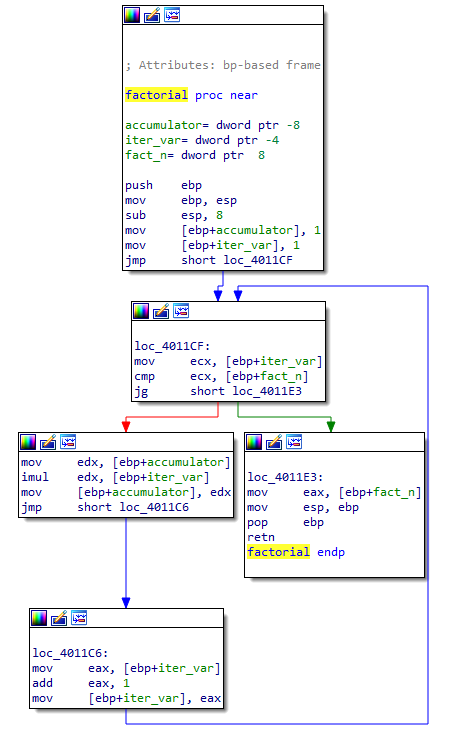
\includegraphics[height=\textwidth,keepaspectratio]{./media/ida}
}
    \caption{An example of a factorial program disassembled with IDA.}
    \label{fig:ida}
\end{figure}

\subsection{Microsoft Visual Studio Debugger}
Microsoft Visual Studio is an Integrated Development Environment. It packs
together many tools that help develop programs for the Windows Operating
System. It mainly supports the C\# and C++ languages. It also has a built-in
debugger. It is both a source and assembly-level debugger.

In figure \ref{fig:msvc}, we show an example of how the GUI looks. On the left
side, we can see the program's source code. The red points are the breakpoints.
The arrow signalizes the current point in the execution. On the right side, we
can see the corresponding assembly. The assembly contains the lines from the
source code to make the mapping between them more apparent. The value and type
of every variable in the scope are displayed on the bottom left. A call stack
is shown in the middle, currently only having main and factorial calls and
locations from where those calls happened. On the right side, values in
registers can be seen. This is only a basic overview of the features, as there
are many more.

\begin{figure}
    \centering{
    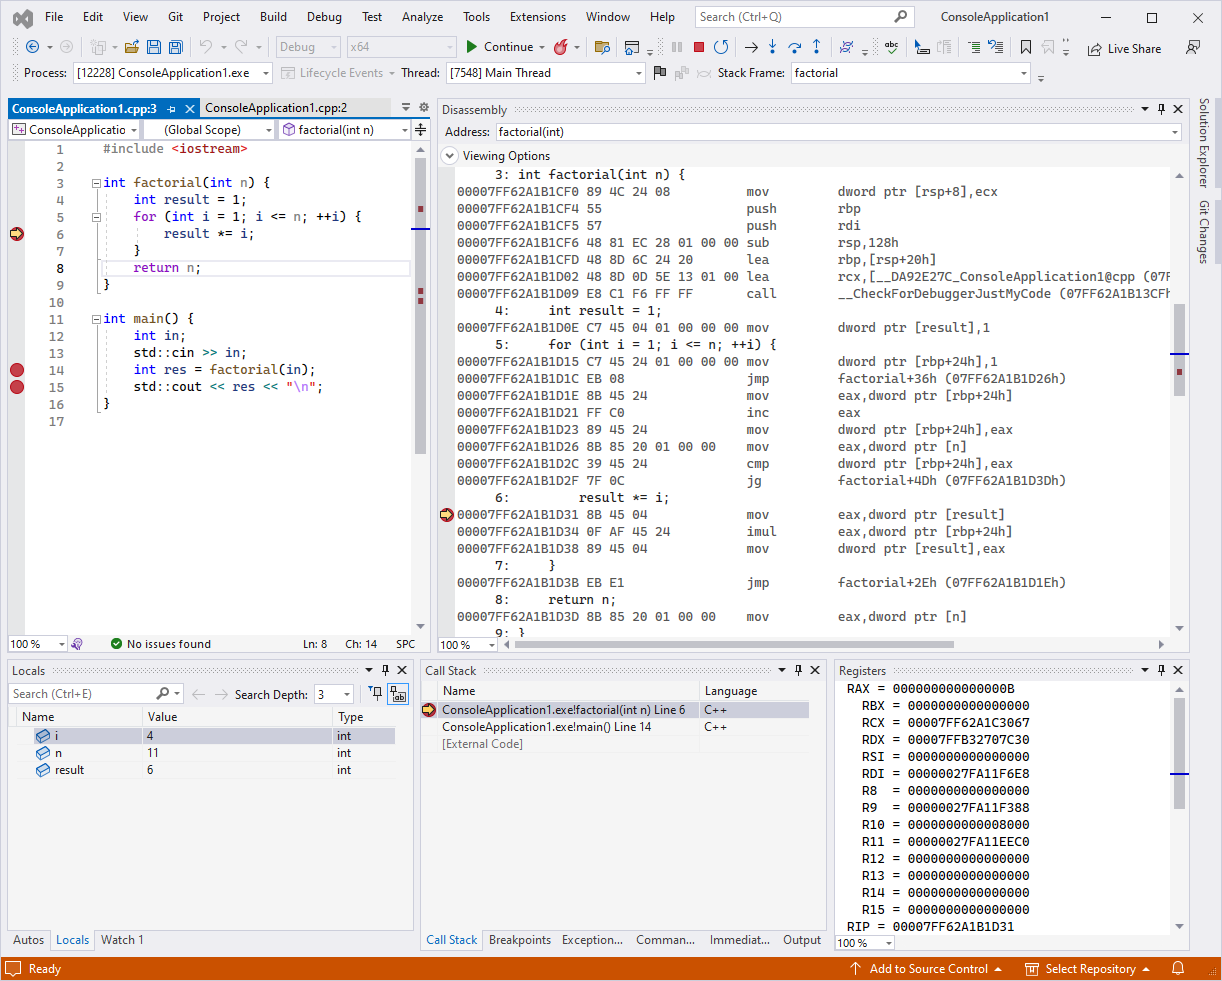
\includegraphics[width=\textwidth,keepaspectratio]{./media/msvc-debugger}
    }
    \caption{An example of debugging factorial program with MSVC debugger.}
    \label{fig:msvc}
\end{figure}

\subsection{LLDB}\label{section:case-study}
In this section, we go into more significant details about the LLDB~\cite{lldb}
debugger. It is a part of the LLVM tools collection~\cite{llvm}. Supported
languages for debugging are the C, Objective-C, and C++ languages (LLVM tools
support mainly those three languages) on desktop and iOS devices. It works
closely with the Clang compiler, which is also part of LLVM, and the LLVM
disassembler. Thanks to this, it stays very up-to-date with current C++
standards. The source code is kept modular with a plug-in architecture. LLDB is
both a source and instruction-level debugger.

LLDB offers an API through which one can interact with the debugger. For
example, the command line application through which one can use LLDB uses this
API. LLDB is written in modern C++, but a bridging interface to the API is
provided for Python. Thanks to this, one can use LLDB for debugging and, for
example, as a library to disassemble machine code~\cite{lldb}.

LLDB provides a command line interface (CLI) through which one can use the
debugger directly. The CLI provides a variety of commands that one can use.
Some examples include
\begin{itemize}
    \item \texttt{process launch} - Starts the debuggee.
    \item \texttt{process attach --pid 123} - Attaches to the process with PID
        123.
    \item \texttt{thread step-in} - Source level single step in currently selected thread.
    \item \texttt{thread step-inst} - Instruction level single step in currently selected thread.
    \item \texttt{thread until 12} - Run until line $12$ is hit or the current
        function returns in currently selected thread.
    \item \texttt{breakpoint set --name foo} - Set breakpoint on all functions
        named \texttt{foo}.
    \item \texttt{breakpoint enable 1} - Enable breakpoint $1$.
    \item \texttt{watchpoint set variable x} - Watch a variable \texttt{x} for
        any writes.
\end{itemize}
All commands are of the following structure:
\begin{lstlisting}
<noun> <verb> [-options [option-value]] [argument [argument...]]
\end{lstlisting}
Some of the commands have shorter forms, like \texttt{step} for \texttt{thread
step-in}. Using an unambiguous prefix works as well, like \texttt{br s -M foo}
for \texttt{breakpoint set --name foo}.

The LLDB debugger has an expression parser. While debugging, one can write an
expression, and the debugger interprets that expression and prints the result
back. An example of usage can be to look at some value in an \texttt{std::map}
structure, which can be achieved by using the \texttt{frame variable
map\_var["Value"]} command. The debugger uses Clang, the C++ compiler, for
parsing expressions. This can be used in conjunction with backticks in
commands. For example, the \texttt{register write rax `loc`} command will write
the value of variable \texttt{loc} into the register \texttt{rax}.

\chapter{Tiny x86}\label{section:T86}
At the FIT CTU, in the NI-GEN course, students have to write a compiler. The
Tiny x86 (T86) architecture was created to make code generation easier. This
allows the students to focus on more interesting parts of compiler design, such
as optimizations. To be able to execute programs written using this
architecture, a virtual machine was created. This was all done as a part of a
master's thesis made by Ivo Strejc~\cite{ivo2021tiny}. This chapter explores
said architecture and the virtual machine. It also delves into the existing
debugging capabilities of said virtual machine.

\section{The T86 Instruction Set Architecture}
The primary goal of the T86 architecture is to be an educational one. The
Virtual Machine made for the ISA allows configuring the number of registers,
the RAM size, or the length of each instruction. This allows the students to
develop their compilers incrementally.

The T86 uses a Harvard architecture, meaning the data and instructions are
physically separated. Memory is addressable by 64-bit blocks, not by 8-bit
blocks, as is the custom in modern computers. It shares some of the registers
we saw on x86-64: the program counter (PC), the stack pointer (SP), the base
pointer (BP), and the flags register. The intended roles for these registers
are the same as on x86-64 architecture. It also has other general-purpose
registers. As previously said, the amount of these is configurable. The
registers stores 64-bit values. It also has float registers, which can store
64-bit float values. These are separated from the standard registers, similarly
to x86-64.

The addressing modes, or what kind of operands instructions can have, include
immediate values, registers, and memory accesses. They can also be combined in
various ways, like \texttt{[R0 + R1 * 2]}, or \texttt{[R0 + 10 + R1 * 2]}. The
addressing modes are, however, not arbitrary, \texttt{[R0 + R1 + R2]} is not a
correct addressing mode for any instruction in the T86 architecture. The
allowed addressing modes also change for each instruction. For example, the
\texttt{MOV} instruction allows a vast range of addressing modes, while the
\texttt{PUSH} instruction only allows a register and an immediate number. For a
full list, refer to~\cite{ivo2021tiny}. The instructions that are taken over
from x86-64 often have more restrictive addressing modes than in x86-64. For
example, the \verb|add| instruction can take a memory offset as a destination
operand in x64-86, but in T86, it can only take registers.

Other than that, the ISA is mainly a subset of the x86-64 most used
instructions, many of which we have already seen in various examples throughout
the thesis. Interesting exceptions are the IO instructions - \texttt{PUTCHAR}
and \texttt{GETCHAR}, which allow for very primitive input and output handling.
Also, a \texttt{DBG} and \texttt{BREAK} instructions are defined. These are
used for debugging, but in a very different way than we have seen in previous
sections. We will touch upon them when discussing the virtual machine
implementation since they are very much tied to it. A small sample of a T86
program can be seen in figure~\ref{fig:t86-example}.

\begin{figure}
    \begin{lstlisting}
MOV  R0, 1
MOV  R1, 50
ADD  R0, R1
MUL  R0, 5
HALT
    \end{lstlisting}
    \caption{A small example of a program in the T86 architecture.}
    \label{fig:t86-example}
\end{figure}

\section{T86 Virtual Machine}\label{section:t86-vm}
The primary objective of the virtual machine is to replicate the CPU as
accurately as possible, without prioritizing execution speed. For instance, the
virtual machine simulates the out-of-order technique briefly described in
section~\ref{section:superscalar-cpu}. The purpose of the virtual machine is to
allow the students to gain a deeper understanding of the effects of pipeline
stalls and similar events on program speed. The virtual machine is able to
generate statistics that provide information about these factors and how
much they influenced the speed of the generated program.

The virtual machine (VM) is implemented in C++, using the newer standards up to
C++17. The VM offers only a single interface, and that is the
\texttt{ProgramBuilder}. This is a class through which one may construct a
program for the T86 VM. An example of how to use this class is in
figure~\ref{fig:t86-intro}. Currently, there is no other way for users to run
programs in the VM. This means that the students are tied to the C++ language,
or use some bindings if they want to use other language.

The \texttt{Cpu} class is the backbone of the interpreter. It is responsible
for running the program. It has a \texttt{halted} function, which returns true
if the \texttt{Cpu} executed a \texttt{HALT} instruction. The \texttt{tick}
performs one tick of the CPU. This does not mean that one instruction gets
executed. The \texttt{Cpu} simulates a superscalar CPU, so one tick is one move
in the pipeline. The \texttt{while} loop in the figure~\ref{fig:t86-intro}
shows to run a T86 program via the \texttt{Cpu} class.

\begin{figure}
    \begin{minted}{cpp}
        ProgramBuilder pb;
        pb.add(MOV{Reg(0), 50);
        pb.add(PUTCHAR{Reg(0)});
        pb.add(HALT{});
        auto program = pb.program();
        Cpu cpu;
        cpu.start(std::move(program));
        while (!cpu.halted()) {
            cpu.tick();
        }
    \end{minted}
    \caption{Simple example of how to create and run a simple program using the
    T86 virtual machine.}
    \label{fig:t86-intro}
\end{figure}

\subsubsection{Debug Instructions}\label{section:t86-debug-cap}
The VM offers some limited debugging capabilities. It has the \texttt{DBG} and
\texttt{BRK} instructions. The \texttt{DBG} instruction takes as an operand a
function. The function has the following signature: \texttt{void fun(Cpu\&)}.
This function then gets executed when the instruction is hit. This can prove
helpful in inspecting the internal state of the CPU. In
figure~\ref{fig:t86-debug}, we show a possible usage of this instruction. The
\texttt{BRK} instruction works similarly. It, however, has no operand. Instead,
a function must be provided before execution to the CPU itself. \texttt{BRK}
then always runs this function when hit.

\begin{figure}
    \begin{minted}{cpp}
    pb.add(DBG{[](Cpu& cpu) {
        if (cpu.getRegister(Reg{0}) == 0) {
            std::cerr << "Register 0 is set to zero!\n";
        }
    });
    \end{minted}
    \caption{Adding a \texttt{DBG} instruction into the T86 program using the
    \texttt{ProgramBuilder}.}
    \label{fig:t86-debug}
\end{figure}

Such debugging capabilities can be helpful but quickly prove insufficient. For
example, when a step-by-step inspection is sought, a debug instruction must be
placed at every second line of the program. Also, interactivity is not present.
However, this function can accept input, so one could create a robust enough to
handle register and memory writing. An idea of how this could be done is
illustrated in~\ref{fig:t86-pocket-debugger} via the \texttt{BRK} instruction.

\begin{figure}
    \begin{minted}{cpp}
    cpu.connectBreakHandler([](Cpu& cpu) {
        char command;
        std::cin >> command;
        if (command == 'c') return; // continue
        else if (command == 'r') { // Read register
            int num;
            std::cin >> num;
            int regval = cpu.getRegister(num);
            std::cerr << std::format("Register {} = {}\n",
                                     num, regval);
        } else if (command == 'w') { // Write register
            int num;
            int val;
            std::cin >> num >> val;
            cpu.setRegister(Reg{num}, Reg{val});
        }
        ... // Other commands
    });
    \end{minted}
    \caption{Small debugger implementation using T86 \texttt{BRK} instruction,
    abbreviated.}
    \label{fig:t86-pocket-debugger}
\end{figure}

This still leaves much to be desired. Not to mention placing the debug
instruction can prove very bothersome.

\chapter{Implementation}
In this chapter, we describe how we went about the implementation of the
debugger and reason about the design choices we made. Also, we describe which
parts of the virtual machine were modified or added to allow the
implementation of the debugger.

\section{T86 ISA Extensions}\label{section:parser}
In chapter~\ref{section:t86-vm}, we showed how to build a program for the T86
VM with the existing builder interface. To allow the usage of other programming
languages, we have created an ELF-like format for the T86 executables. The
format is a text one, making it easy to use. An example of a program in said
format is shown in figure~\ref{fig:t86-program}. It is very similar to the
assembly we have shown in previous sections. Thanks to this, students can
implement their compiler in any programming language they want and emit the T86
program in this format as a text file. An unfortunate side effect is that we
can no longer use the \texttt{DBG} instruction. However, the debugger we will
later present will be much more powerful than the \texttt{DBG} instruction.

As can be apparent from the example, we also use sections. The \texttt{.text}
section is the only mandatory one. It contains the instructions that will be
executed. Another one is the \texttt{.data} section. Here, either raw numbers
or strings can be written. The contents of this section are then loaded by the
VM and stored into the memory, beginning at memory cell 0 and upwards. There
are also debug sections, which we will present when discussing debugging
information.

\begin{figure}
    \begin{lstlisting}
.data
"Hello, World!\n"

.text
0   MOV [BP - 1], 0
1   JMP 8
2   MOV R0, [BP - 1]
3   MOV R1, [R0]
4   PUTCHAR R1
5   MOV R0, [BP - 1]
6   ADD R0, 1
7   MOV [BP - 1], R0
8   MOV R0, [BP - 1]
9   CMP R0, 13
10  JLE 2
11  HALT
    \end{lstlisting}
    \caption{Example of an T86 program which prints "Hello, World!".}
    \label{fig:t86-program}
\end{figure}
We will also add two new instructions. First is the \texttt{PUTNUM}
instruction, which prints the numerical value in the register and a newline.
This is intended as a very primitive debug instruction and to ease the
automated testing of the compiler. The only other way of output was to print a
char which was represented by the ASCII value. With this instruction, students
can bootstrap and test the basic implementation of their compiler more easily.

Another one is the \texttt{BKPT} instruction. This instruction is similar to
the \texttt{INT3} instruction from x86-64 or the \texttt{BKPT} instruction from
ARM. It is a software breakpoint. The virtual machine has no support for
interrupts, which are needed for debugging to work. This will be the focus of
the next section.

\section{T86 Debugging Support}
We could bake the debugger into the virtual machine itself, which would likely
be the simplest way to implement it. However, the goal of the debugger is not
only to ease the code generation part but to be a learning point so that
students might grasp how a real debugger works\footnote{The VM followed the
same philosophy.}. Because of this, we aim to simulate the real-world debuggers
as closely as possible. The compilers may also have more targets in the future,
not just the T86 VM. If we made the debugger part of the T86 VM, we could not
use it for a possible new virtual machine. In conclusion, the virtual machine
and the debugger will be two entirely different programs and as such, two
completely different processes.

In the debugger implementation for Linux, the subject of section
\ref{section:linux-dbg}, we described how an operating system's kernel allows
the debugger's implementation via a specific API. There is no operating system
between the virtual machine and the program. Still, we will strive to make the
API similar to the ptrace API. The debugger and the VM will have to communicate
together somehow. For interprocess communication, there are several
possibilities.

Both the VM and the debugger use an abstract class representing an interface
that provides two methods, \texttt{Send} and \texttt{Receive}. The
implementation of this interface then handles the concrete way of
communication. The debugger and VM do not care about it; they merely use these
two methods. There are currently two implementations of this interface. One is
using network communication through sockets. This way, the debugger may attach
to an existing process, even on an entirely different computer. It, however,
has a disadvantage. The messages sent are often short and we need to send a lot
of them. This proved too slow, even with few messages being sent. The second
implementation is via threads. The debugger runs the VM in another thread, and
they communicate via shared queues. This is far faster and allows the debugger
to run the process by himself, making it easier to use and behave like
real-world debuggers.

The format of the communication is a text one, merely because of the ease
of use as opposed to binary format, it is also clearer to see what is
happening. The commands that the virtual machine API offers are
\begin{itemize}
    \item \texttt{PEEKREG x} - Return values of all normal registers.
    \item \texttt{POKEREG x y} - Set the value in register \texttt{x} to
        \texttt{y}.
    \item \texttt{PEEKFLOATREG} - Return values of all float registers.
    \item \texttt{POKEFLOATREG x y} - Set the value in float register
        \texttt{x} to \texttt{y}.
    \item \texttt{PEEKDEBUGREG} - Return value in all debug registers.
    \item \texttt{POKEDEBUGREG x y} - Set the value in debug register
        \texttt{x} to \texttt{y}.
    \item \texttt{PEEKDATA x cnt} - Return value in memory at addresses $x$ to $\texttt{x} + \texttt{cnt} - 1$.
    \item \texttt{POKEDATA x y} - Writes a value \texttt{y} into a memory at
        address \texttt{x}.
    \item \texttt{PEEKTEXT x cnt} - Return instruction from \texttt{x} to $\texttt{x} + \texttt{cnt} - 1$.
    \item \texttt{POKETEXT x INS} - Rewrite the instruction at address
        \texttt{x} with the newly supplied instruction.
    \item \texttt{CONTINUE} - Continue the execution.
    \item \texttt{TERMINATE} - Stop the execution, terminating the virtual machine.
    \item \texttt{REASON} - Get the reason why the program stopped (breakpoint,
        singlestep, halt...).
    \item \texttt{SINGLESTEP} - Do native level single step.
    \item \texttt{TEXTSIZE} - Return the size of the program.
\end{itemize}

An example of how those commands can be used for communication between the
virtual machine and the debugger is shown in figure~\ref{fig:dbg-vm-seq}. The
interface is similar to basic ptrace commands. If the command should not return
anything, the VM sends back an \texttt{OK} message. We separate the memory and
instruction writing because T86 uses Harvard architecture, whereas Linux does
not separate text and data address spaces~\cite{ptrace}, so the two requests
were equivalent there. The API is made to be simple on purpose. Anything more
complex should be handled in the debugger itself.

\begin{figure}
    \centering
    \scalebox{0.8} {
    \begin{tikzpicture}
        \draw (0,0) -- (0,-20.2) (7,0) -- (7,-20.2);
        \node at (7,.3) {Debugger};
        \node at (0,.3) {Virtual machine};
        \draw[<-] (0,-1) -- node[midway,above] {Initializes connection} (7,-1);
        \draw[->] (0,-2) -- node[midway,above] {Accepts connection} (7,-2);
        \draw[<-] (0,-3) -- node[midway,above] {\texttt{"PEEKTEXT 5 1"}} (7,-3);
        \draw[->] (0,-4) -- node[midway,above] {\texttt{"MOV R0, 1"}} (7,-4);
        \draw[<-] (0,-5) -- node[midway,above] {\texttt{"POKETEXT 5 BKPT"}} (7,-5);
        \draw[->] (0,-6) -- node[midway,above] {\texttt{"OK"}} (7,-6);
        \draw[<-] (0,-7) -- node[midway,above] {\texttt{"CONTINUE"}} (7,-7);
        \draw[->] (0,-8) -- node[midway,above] {\texttt{"OK"}} (7,-8);
        \draw[->] (0,-10) -- node[midway,above] {\texttt{"STOPPED"}} (7,-10);
        \draw[<-] (0,-11) -- node[midway,above] {\texttt{"REASON"}} (7,-11);
        \draw[->] (0,-12) -- node[midway,above] {\texttt{"SW\_BKPT"}} (7,-12);
        \draw[<-] (0,-13) -- node[midway,above] {\texttt{"CONTINUE"}} (7,-13);
        \draw[->] (0,-14) -- node[midway,above] {\texttt{"OK"}} (7,-14);
        \draw[->] (0,-16) -- node[midway,above] {\texttt{"STOPPED"}} (7,-16);
        \draw[<-] (0,-17) -- node[midway,above] {\texttt{"REASON"}} (7,-17);
        \draw[->] (0,-18) -- node[midway,above] {\texttt{"HALT"}} (7,-18);
        \draw[<-] (0,-19) -- node[midway,above] {\texttt{"TERMINATE"}} (7,-19);
        \draw[->] (0,-20) -- node[midway,above] {\texttt{"OK"}} (7,-20);
    \end{tikzpicture}
    }
    \caption{A sequence diagram for the communication between the virtual
    machine and the debugger. If the label is enclosed in quotes, it is the
    actual text message that is being sent.} \label{fig:dbg-vm-seq}
\end{figure}

The \texttt{Cpu} class, which we have described in section~\ref{section:t86-vm},
has no support for interrupts. The \texttt{halted} method is kind of similar
to interrupts, but only allows for signaling the \texttt{HALT} instruction
execution. We need more than that.

We added another manager-like class called \textit{OS}. This class will take
care of running the program via the \texttt{Cpu} class. We also added an
\textit{interrupt} capability to the \texttt{Cpu}. To check if and which
interrupt happened, the \texttt{Cpu} now provides a function, similar to the
\texttt{halted} function. The OS calls the \texttt{tick} method periodically,
and after every tick, it checks if a halt or interrupt occurred. If it did,
then it passes it to some handler. When interrupt happens, unrolling must be
done to display proper values in registers and memory. This was described in
section \ref{section:superscalar-cpu}. The unrolling mechanism was fortunately
already implemented by the T86 VM author. It was used for the \texttt{DBG} and
\texttt{BRK} instructions, and we can use the same mechanisms for our addition
of interrupts.

The \texttt{BKPT} instruction we added is used for software breakpoints.
Executing this instruction causes an interrupt \texttt{3} to occur. It is also
possible to set a special flag that causes the \texttt{Cpu} to send the
interrupt \texttt{1} after every executed instruction. When an interrupt that
is caused by some debugging features happens, the \texttt{OS} calls a method
in the \texttt{Debug} class. This class is also a new addition and is
responsible for communication with the debugger. It uses the text protocol we
mentioned previously.

We also added debug registers. These are a special type of registers designed
for triggering breaks on memory access. There are a total of five debug
registers, with the first four containing the memory cell addresses. The fifth
register, called the control register, contains four bits that indicate the
status of each of the first four registers. If a register is active and the
program writes to a memory cell with the same address as is stored in the
register, an interrupt \texttt{2} is generated. Furthermore, the control
register's bits from 8 to 11 reveal which register caused the interrupt. For
instance, if bit 10 is set to 1, the third register is responsible for the
interrupt and the address stored in that register is the one that was written
into.

\section{Native Debugger}
The implementation is done in the C++ language. It uses newer standards up to
the C++20 standard. The debugger is implemented as a library. We will call this
the backend of the debugger. A command line interface was also developed,
through which the users might interact with the debugger. This will be called
the frontend of the debugger.

The implemented debugger consists of two main parts. The first one aims to
support native (instruction) level debugging. This part work without
\textbf{any} debugging information whatsoever. The second part focuses on
source-level debugging, and is described in
section~\ref{section:source-debugger}.

The native debugger is split into two additional layers to make it more
modular. The first layer is called a \texttt{Process}. It is an interface
representing the debuggee process. The implementation of this interface is
responsible for dealing with the concrete architecture, the API of that
architecture, and the communication with the debuggee. One implementation is
provided for the T86 VM. For instance, it has a method called \texttt{ReadText}
and \texttt{WriteText}. The internals of these methods use the
\texttt{PEEKTEXT} and \texttt{POKETEXT} API we described. Outside of this
class, the communication API is never used. If, in the future, another virtual
machine is made, for whichever architecture, it is only needed to implement
this interface. The rest of the debugger can be used as-is.

Another layer is the \texttt{Native} class, which implements the complicated
logic behind a debugger, like setting a breakpoint, handling single-step, and
so forth. It is the primary bread and butter of the native part of the
debugger. Most algorithms are similar to the Linux debugger implementation
presented in section \ref{section:linux-dbg}. For illustration, in figure
\ref{t86dbg:breakpoint} we show a snippet of code used to create a breakpoint.
It first reads the text at the address where we want to set the breakpoint. The
breakpoint opcode then rewrites this text, and the backup of the text is
stored.

When we arrive at the breakpoint and want to continue further, we need to unset
the breakpoint, i.e., replace the breakpoint opcode in the T86 program with the
backup we saved, do a native-level single step, and write the breakpoint back.

Since breakpoints change the underlying code of the debuggee, we need to be
careful when presenting information to the user. If we printed the text that we
get from the debuggee, it might contain the \texttt{BKPT} instructions we set
earlier. We need to mix it with the backup code stored in breakpoints to show
the assembly of the program correctly.

The Native class uses a \texttt{DebugEvent} structure which indicates what
caused the VM to stop. It is implemented as a \texttt{variant} of multiple
structures, for instance, the \texttt{BreakpointHit} or the
\texttt{WatchpointTrigger} structure. It is a variant because the watchpoint
also needs to convey information about an address that caused the break, as do
breakpoints. It could also signal if the break was caused by reading or writing
to the memory cell, although for now, the T86 VM only interrupts on writing.

\begin{figure}
    \begin{minted}{c++}
SoftwareBreakpoint CreateSoftwareBreakpoint(uint64_t address) {
    auto opcode = GetSoftwareBreakpointOpcode();
    // Read the text at the breakpoint address
    auto backup = process->ReadText(address, 1).at(0);
    // Rewrite it with the breakpoint opcode
    std::vector<std::string> data = {std::string(opcode)};
    process->WriteText(address, data);
    // Check that it was truly written
    auto new_opcode = process->ReadText(address, 1).at(0);
    if (new_opcode != opcode) {
        Error(...);
    }
    // Create a breakpoint object which keeps the text backup
    return SoftwareBreakpoint{backup, true};
}
    \end{minted}
    \caption{Debugger code in the \texttt{Native} class to enable a breakpoint.}
    \label{t86dbg:breakpoint}
\end{figure}

The native debugger has the following features:
\begin{itemize}
    \item Breakpoints - Can set, unset, enable and disable software breakpoints.
    \item Watchpoints - Can set and unset watchpoints on memory writes.
    \item Single stepping - Can do native level step into, which executes
        current instruction, out, which runs the program until it leaves
        current function and over, which treats function calls as a single
        instruction.
    \item Text manipulation - Can read and write into the debuggee text area,
        effectively allowing to overwrite the running code.
    \item Data manipulation - Can read and write into the program memory area.
    \item Register manipulation - Can manipulate with normal, float and debug registers.
\end{itemize}

\section{Debugging Source Code}\label{section:source-debugger}
With the solid foundation represented by the native part of the debugger, we
can extend it by providing some form of source-level debugging. For this part,
we need to remember that the debugger will only be used by students. As such,
we ought to have gentler debugging information than DWARF, but we certainly can
take inspiration from it.

As we previously mentioned, the executable with T86 code is separated into
sections. The \texttt{.text} and \texttt{.data} sections are for the VM. We
will introduce new sections where debugging information will be stored. All
those sections will have \verb|.debug_| prefix. The simplest new section is
\verb|.debug_source|, which should contain the original source code which was
compiled into this executable. This later allows us, with the combination of
other information, to display the source code lines.

The main philosophy of the source-level debugger is to allow an arbitrary
amount of debug information. For instance, the user can generate information
about one function only, and for that function, source debugging capabilities
will work, but not for any other. This means that users can generate debugging
information incrementally.

In the NI-GEN course, students are creating compilers from the TinyC language.
This is a small subset of the C language. It has simpler grammar and only
following types: \texttt{int}, \texttt{double}, \texttt{char}, pointers,
structured types, and static arrays. We aim to support all of TinyC language in
our source layer of the debugger.

The debugger is, however, not only limited to TinyC language. Any imperative
language that can be encoded with the following debugging information is
suitable to be debugged at the source level. We show an example of this in a
provided test case for the debugger where we debug the LLVM IR. It can be found
as an attachment to the thesis on path \texttt{impl/src/dbg-cli/tests/llvm.ir}.
We also provide a documentation for developers who wish to generate this
debugging information in the thesis attachment on path
\texttt{impl/docs/source-info.md}.

The logic behind the source level debugging is mostly handled by the
\texttt{Source} class. It also stores all of the source level mapping, which we
are about to describe below. Some of the methods work closely with the
\texttt{Native} class to achieve functionality. That shouldn't be suprising, as
we said, source-level debugging is built upon native-level debugging.

\subsection{Line Information and Source Code}
The line information is encoded in a table, where every row is:
\texttt{<line>:<address>}. This is far simpler than the DWARF way which we
described in section~\ref{section:line-number-information}. We do not care
about being space efficient, so we did a table instead of virtual machine
specification. We also feel like this should be an entry level debugging
information, so that students are not discouraged outright. It misses some
information that DWARF had, like columns. It still however proves quite
sufficient for most cases. The information should be stored in the
\verb|.debug_line| section.

With this information, we are able to do source-level breakpoints. If the
source code is also provided, we can show the user on which line is the
debugged program currently paused. It is not necessary to specify every line in
the program. The debugger will refuse to put a source-level breakpoint on some
line if it does not have the necessary information. The source code should be
under the \verb|.debug_source| section, which must be the last section in the
executable.

\subsection{Debugging Information Format}
In the line information, we provided a straightforward format. However, we will
need a more sophisticated structure to describe some advanced constructs of the
source code. We will draw inspiration from the Dwarf Debugging Information
(DIE). Take a look at figure~\ref{fig:t86dbg-die}, which shows an example of
such debugging information. It has a tree-like structure which, in some ways,
mimics the original program. The nodes of this tree are also called debugging
information entries (DIEs). Those entries can have other entries as their
children, and each entry has a tag that is part of its name (for example, the
\verb|compilation_unit| tag). They can also have attributes that describe their
properties. As can be seen, this is very similar to the DWARF debugging
information format. Unlike DWARF, it will be a text format. This allows us to
generate the format easily and to spot mistakes quickly. We don't want the
students to debug their generated debugging information.

For instance, the tag \verb|DIE_function| represents a function. As attributes,
it has a name, beginning address, and end address. With this additional
information, we can set a breakpoint on a function name. We can also display in
which function we are located when a break happens.

It also has one direct child, a \verb|DIE_scope|. The scope entry is mainly
used for keeping track of which variables are currently active because the T86
(or any other assembly language in general) has no notion of scopes. In the
scope entry in the example, only one variable called \texttt{d} exists. Thanks
to those entries, we can list currently active variables. We, however, often
need to examine the value of a variable. To achieve this, information about the
location and the variable type is needed. Global variables should be outside of
a function, as descendants of the \verb|compilation_unit| entry.

\begin{figure}
    \begin{lstlisting}
DIE_compilation_unit: {
DIE_function: {
    ATTR_name: main,
    ATTR_begin_addr: 0,
    ATTR_end_addr: 10,
    DIE_scope: {
        ATTR_begin_addr: 0
        ATTR_begin_addr: 10
        DIE_variable: {
            ATTR_name: d,
        },
    }
}
}
    \end{lstlisting}
    \caption{Debugging function information for the T86 debugger.}
    \label{fig:t86dbg-die}
\end{figure}

The type information is encoded as a standalone DIE. Currently, three type
entries are present, one for primitive types (\texttt{int}, \texttt{double}, or
\texttt{char}), one for pointers, and one for structured types (\texttt{struct}
or \texttt{class} in C++). Other types can be easily added in the future. The
types are saved as separate entries, and as such, we need some way to link them
together with the variables. We will use the \verb|ATTR_id| attribute to
achieve this. This attribute should be unique for every entry, having similar
role to the \texttt{id} attribute of HTML elements~\cite{html4}. The variables
themselves have the \verb|ATTR_type| attribute, which will have an id of the
type as its value. An example of a pointer type that points to an int type is
in figure~\ref{fig:t86dbg-types}. If we had a variable that is a pointer to
int, it would need to have the \verb|ATTR_type: 1| attribute because the id of
a pointer type to integer is one.

The primitive types need to have their size. For T86, this is the number of
memory cells it occupies, which will almost always be one since one memory cell
is 64 bits. It also has a name for its primitive type. Currently, three
are supported:
\begin{itemize}
    \item \texttt{int} - A signed integer.
    \item \texttt{float} - A floating point number.
    \item \texttt{char} - A number representing an ASCII character.
\end{itemize}

Additionaly, we also support pointer types (including pointers to pointers),
static arrays and structured types, which are a bit more complicated. They need
to have a list of members which are stored in the structure. For each member,
an offset from the beginning of the structure must also be specified. It also
must provide a size because the compiler might align it, and it may be larger
than the sum of the size of its members.

\begin{figure}
    \begin{lstlisting}
DIE_primitive_type: {
    ATTR_name: int,
    ATTR_id: 0,
    ATTR_size: 1,
},
DIE_pointer_type: {
    ATTR_type: 1,
    ATTR_id: 1,
    ATTR_size: 1
},
    \end{lstlisting}
    \caption{Debugging type information for the T86 debugger, showing an
    \texttt{int} primitive type and a pointer to \texttt{int} type.}
    \label{fig:t86dbg-types}
\end{figure}

With this information, we can show the type of a variable. Nevertheless, the
most valuable thing is its value. Variables are either stored in memory,
registered, or optimized out completely. We will follow DWARF's footsteps and
provide a virtual machine specification.

The virtual machine is stack-based one. After all instructions are executed,
the value at the top of the stack represents the resulting location. It can
either be a register or an memory offset. We offer several examples of programs
for the virtual machine:
\begin{itemize}
    \item \texttt{PUSH R0} - Pushes the register \texttt{R0}. No instructions
        remain, so the resulting location is the \texttt{R0} register.
    \item \texttt{PUSH BP; PUSH -2; ADD} - Pushes the \texttt{BP} register and
        the \texttt{-2} offset onto the stack. The \texttt{ADD} instruction
        pops two values from the stack and adds them together. If the value is
        a register, the value that is stored in that register is taken. The
        result from the addition is pushed back onto the stack.
    \item \verb|BASE_REG_OFFSET| - Does the exact same chain of operations as
        the previous example. Since the variables are often stored in memory at
        some offset from the base pointer, we provide this short hand.
\end{itemize}

There is also a dereference instruction, which dereferences a value in memory.
That can be useful for tracking location of pointed variables. This virtual
machine is also easily extendable. With this kind of power, the location of
variables can almost be arbitrary and not only tied to a register or an offset
from the base register. This information is stored in a variable entry
attribute called \texttt{ATTR\_location}. If all this information is provided,
we know where the variable is stored and may look up its value. Together with
the type information, we might also properly interpret the value and report it
to the user.

\subsection{Source Expressions}
We could make a very straightforward implementation of getting variable value
by its name. It is only a matter of finding the variable entry with the correct
name and interpreting its location and type. However, we often need to inspect
some more complicated expressions. For example, we may want to display some
struct member or a value at which pointer points.

The debugger has a built-in interpreter for such expressions. It builds an AST
from the expression and interprets it using an
AST walk~\cite{crafting-interpreters}. The AST interpreter leverages the
\texttt{Native} class to fetch variable values. The interpreter supports almost
all C operators, including the assignment operator. It, however, has stricter
typing than C. An example of such an expression is \texttt{foo[2]->bar + 3}.
This is a very powerful feature, as it allows one to easily inspect or modify
various variables or expressions. If a user wishes to modify part of an array,
there is no need to use the raw memory or register setters. Instead, it is
possible to write \texttt{array[x] = y}.

The AST nodes are distinguished by types. They also need to store the location
of the expression  if it is an expression that can appear on the left-hand
side of the assignment operator. Examples of expressions that must store the
location: \texttt{a}, \texttt{*(a + 1)}, \texttt{a[5]}, while the following
expressions do not have any locations because they cannot appear on the left
side of the assignment operator: \texttt{a + 1}, \texttt{5}, \texttt{array[0]
* y}.

\section{Frontend}
We provide two command line interface programs. First one is for the T86, is
runs the given T86 program on the virtual machine. The second application
leverages the debugger library to create a command line interface for the
debugger. It provides many commands, and its manual can be found in the thesis
attachment under path \texttt{impl/docs/debugging.md}. In this file, a table
can be found showing how some of the commands the application accepts differ
from the GDB debugger.

The main priority of the CLI is to make the debugger easy to use. It consists
of several commands, one of them is \texttt{breakpoint set 5}, which will set a
source-level breakpoint on the fifth line of the program. It is, however, not
necessary to write the whole command. Any prefix will do, like \texttt{b s 5}.
The CLI leverages the \textit{linenoise}~\cite{linenoise} library to make the
REPL satisfying to use.

The CLI also displays various information on program stop, like why the program
stopped, on which address or line, and prints the surrounding lines of assembly
or source. The CLI can also list breakpoints and display their locations in the
disassembly or the source code. Figure~\ref{fig:cli-hit} provides an example of
a breakpoint hit report. The debugger had all debugging information available
here. It can show the line in the source code where the breakpoint happened,
name the offending function, and variables in scope.

When variable values are printed, the format tries to accomodate their type.
For example, variables that are arrays or pointers to the \texttt{char} type
print the value of the variable as a string literal.

\begin{figure}
    \begin{lstlisting}
Process stopped, reason: Software breakpoint hit at line 11
function main at 7-18; active variables: a, b
      9:    int b = 6;
     10:    swap(&a, &b);
@->  11:    print(a);
     12:    print(b);
     13:}
    \end{lstlisting}
    \caption{Example of the debugger CLI reporting a breakpoint hit.}
    \label{fig:cli-hit}
\end{figure}

\chapter{Evaluation}
This chapter aims to assess the effectiveness of the debugger. Speed is
measured to evaluate whether the debugger has any performance impact when
debugging standard and computative demanding programs. We also evaluate its
feature richness and ease of use, comparing it to modern state-of-the-art
debuggers like the GDB.

\section{The development process}
The development of the thesis was done in a GitHub repository. The power of
Github was leveraged not only for keeping history but also for recording
issues, planning the development, or ensuring that the repository is in a
consistent and working state via GitHub actions, which runs tests before a pull
request is accepted. The actions run on two operating systems, Ubuntu and
MacOS, ensuring the project works on both.

The project itself contains many tests. The code is first tested via many unit
tests using the \texttt{GoogleTest} framework. The unit tests cover almost all
parts of the code. It also has integration tests for T86-CLI and the debugger
CLI. Another student\todo{citace} created a TinyC to T86 compiler as part of
his thesis. He was kind enough to send the implementation to us so that we
could generate various tests more easily. As a result, most of the integration
tests were generated by the said compiler.

\section{Usage and user testing}
We followed the interface of the GDB closely so that the users were familiar
with the debugger before even running it. However, we choose to diverge on some
of the features. For example, the GDB uses the \texttt{stepi} command for
single stepping. This form has a common prefix with the \texttt{step} command.
We, however, expect our users to use assembly-level debugging more often than
source-level debugging, so we choose the \texttt{istep} command form instead.
The two commands have no shared prefix, so typing \texttt{is} is enough.

Also, the program is run via \texttt{run}, this starts the VM, but the program
is paused. In GDB, one has to use the \texttt{start} command to get equivalent
behavior, \texttt{run} runs the program without stopping at the beginning. When
we did a brief user testing, it wasn't very clear to the user. However,
renaming the command \texttt{run} to \texttt{start} would cause it to have the
same prefix as \texttt{step}. Considering this, we've decided to leave the
command as \texttt{run}.

There are other minor things; most of them come from the fact that we
prioritize assembly-level debugging, whereas GDB focuses more on the source
level. We provide a short list of examples showing how to achieve something in
GDB and our debugger \todo{Linknout path do sourcu nebo to pridat sem jako
appendix}.

One student already tested the debugger and said the experience was quite
pleasant. There were a few minor things that he didn't like and offered
solutions for (for example, the usage message can only be displayed after the
debuggee program is executed, meaning the \texttt{run} command must be invoked
first), most of which we took to heart and corrected. Additionally, the student
that provided us with the TinyC compiler used the debugger to debug the code
his compiler generated. A talk about how is the repository used in production
by students.\todo{complete this part when code is public}.

\section{Performance}
The performance of the debugged program can suffer. In this section, we show
which debugging features hurt performance the most and if there is any way
around it. The tests were done on two programs: a quicksort~\cite{quicksort}
algorithm and a naive prime number checker\todo{Include the source code here?
Both the T86 and TinyC}. The difference between those two programs is that the
quicksort is recursive, whereas the primes are implemented via a loop. The
runtime of those two programs on the virtual machine alone is similar.

\begin{table}[]
\centering
\begin{tabular}{||c c c||}
\hline
Test Case & Quicksort - Time & Prime numbers - Time \\
\hline\hline
1. & $9.96$            & $11.68$  \\
2. & $9.32$            & $12.33$  \\
3. & $10.9$            & $58.32$  \\
4. & $10.9$            & $72.85$  \\
5. & $9.73$            & $10.53$  \\
6. & $9.65$            & $230.81$ \\
\hline
\end{tabular}
\caption{Performance comparison when using various features of the debugger.
The Quicksort had $674$ breakpoints hits, while prime numbers had $101266$ hits.
Each case was run five times and average was taken.}
\label{table:benchmark}
\end{table}

We will measure the speed on the following cases:
\begin{enumerate}
    \item Run the VM without the debugger.
    \item Connect the debugger and immediately invoke the \texttt{continue} command.
    \item Connect the debugger and set breakpoint at hot spot of the program.
        For quicksort, this will be the main recursive function. For primes,
        it will be the body of the loop. When the breakpoint is hit invoke
        the \texttt{continue} command.
    \item Same as before, but at every breakpoint, hit read a $100$ cells of
        memory and the \texttt{IP} register.
    \item  Step over a computationally expensive function. For quicksort, it is
        the \texttt{quicksort} function; for primes, it is the \verb|is_prime|
        function.
    \item Set a breakpoint in the most expensive function and run the program.
        Remove the breakpoint on the first hit and step out of the function.
        The expensive functions are the same as in the previous test.
\end{enumerate}

The results are in table \ref{table:benchmark}. It is apparent that just having
the debugger connected introduces almost no slowdown. In the quicksort case,
the program is even faster. This is probably due to measurement errors. The
breakpoints, however, do cause a slowdown. In the quicksort, the program had
$674$ breakpoint hits, while in the prime numbers, it had $101266$. The
quicksort version is $1.1$ times slower, which is negligible. However, in the
prime numbers test performance takes a severe hit with being at least $5$ times
slower. This shouldn't come as a surprise, as there is an enormous number of
breakpoint hits. The communication between the debugger and the debuggee starts
to slow down the program. Given the circumstances, this result is still
satisfactory. Reading memory and registers together with the breakpoints
introduces minimal slowdown.

The step-over result is not very surprising. It puts a breakpoint after the
call and runs the program, so the result should be roughly the same as case
number one. Step out is stepping over until a return is encountered. This works
well in the recursive function because it skips a large part of the program.
But in the prime case, which is implemented via a loop, it severely slows down
the program because it essentially single steps through the entire thing.

The debugger is more than suited for usage on regular programs. In the case of
very computationally intensive programs, certain debugger features will start
to struggle. On the other hand, a hundred thousand breakpoint hits is an
unpractically large number. We consider the quicksort example as a peak of what
the students will have to debug, and in that example, the debugger had almost
no slowdowns. Still, it is something to keep in mind while using the debugger,
and there is a potential for improvements in the future.

\chapter{Conclusion}
\section{Summary}
We explored debugging capabilities of modern CPU architectures. We also
described how debugging is supported at various layers, from operating systems
to compilers. Then, we discuss the T86 architecture and its insufficient
debugging support. We remedy this by adding a debugging API inspired by modern
architectures. We also created a native and source-level debugger, which is
production ready and already used in the NI-GEN course at FIT CTU. This
debugger is extensible enough that if a new architecture, virtual machine, or
source language comes into play, it should be fairly easy to add support for it
into the debugger.

The debugger encourages students in the NI-GEN course to investigate how the
debugger works, the connection between the generated machine code and the
source code, and to emit information about those connections so that the
debugger can work at the source level. It can also make their lives easier
since the debugger works at the native level without additional work, allowing
them to debug the code their compiler generated.

The tool is, along with the enhanced T86 virtual machine, openly available at \\  
\verb|https://github.com/Gregofi/t86-with-debug|.

\section{Future Work}
There are many possible improvements to be made. We have created a new
executable text format for T86 ISA and, consequently, a parser for that format.
Students, however, have to generate this text, which includes not only the
instructions themselves but also the debugging information. A builder interface
could go a long way, especially for the most commonly used languages in the
NI-GEN course.

The native part of the debugger is fairly complete. It can always be extended
for new architectures and virtual machines should they emerge. The expression
command, which evaluates a TinyC expression, cannot handle function calls.
There is also no way to format the output (for instance, to print an integer as
a hexadecimal number). The expression interpreter can always be extended to
handle other languages.

New types can always be added to the debugging information. For example, we are
missing enums, qualifiers like \texttt{const} and \texttt{mutable}, or more
advanced types that are in the C++ standard library. Those types are not in the
TinyC language that is being taught in the NI-GEN course, but the debugger is
not strictly tied to the language. Some parts of the program could be
optimized, like the step out, which can prove slow, as demonstrated in
section~\ref{section:benchmark}.

The debugger currently does not handle frame information in any way. This could
be a helpful addition so that it displays call frames and allows one to step
out of them. This would require a new section, which would have to contain
enough information to simulate an unwind. The exact mechanism was described in
section~\ref{section:call-frames}.

The T86 VM generates statistics about the program execution. It records things
like pipeline stalls. Since the debugger has the capability to connect the
source to the assembly, it could display the code hot spots in the source code
directly.

Last but not least, a graphical user interface could be created for the
debugger. Currently, it only offers a command line interface. A graphical
interface could be more pleasant to work in. Alternatively, it could be hooked
to an existing editor, like the Visual Studio Code, which allows the usage of
other debuggers like LLDB or GDB.


% WARNING: If something doesn't work, put these guys back
\appendix\appendixinit % do not remove these two commands

\chapter{Nějaká příloha}


Sem přijde to, co nepatří do hlavní části.
 % include `appendix.tex' from `text/' subdirectory

\backmatter % do not remove this command

\printbibliography % print out the BibLaTeX-generated bibliography list

\chapter{Obsah přiloženého média}


	\dirtree{%
		.1 readme.txt\DTcomment{stručný popis obsahu média}.
		.1 exe\DTcomment{adresář se spustitelnou formou implementace}.
		.1 src.
		.2 impl\DTcomment{zdrojové kódy implementace}.
		.2 thesis\DTcomment{zdrojová forma práce ve formátu \LaTeX{}}.
		.1 text\DTcomment{text práce}.
		.2 thesis.pdf\DTcomment{text práce ve formátu PDF}.
	}
 % include `medium.tex' from `text/' subdirectory

\end{document}
